% ~~~~~~~~~~~~~~~~~~~~~~~~~~~~~~~~~~~~~~~~~~~~~~~~~~~~~~~~~~~~~~
%
% CUHK Mathematics
% MATH1030: Linear Algebra I
%
% ~~~~~~~~~~~~~~~~~~~~~~~~~~~~~~~~~~~~~~~~~~~~~~~~~~~~~~~~~~~~~~

\documentclass[a4paper,12pt]{article}
\usepackage{standalone}
% Basic
\usepackage[T1]{fontenc}
\usepackage[utf8]{inputenc}

% ------------------------------------------------------------ %

% Packages
\usepackage{amsmath, amsthm, amssymb}
\usepackage{blindtext}
\usepackage{enumitem}
\usepackage{extramarks}
\usepackage{fancyhdr}
\usepackage[margin=1in]{geometry}
\usepackage{graphicx}
\usepackage{hyperref}
\usepackage{indentfirst}
\usepackage{listings}
\usepackage{mathrsfs}
\usepackage{mdframed}
\usepackage{multicol, multirow}
\usepackage{needspace, setspace}
\usepackage{paracol}
\usepackage{pgf, tikz, pgfplots}
\usepackage{silence}
\usepackage{xcolor}

% ------------------------------------------------------------ %

% Spacings
\newcommand{\n}{\vspace{3mm}} % Context spacing
\newcommand{\s}{\vspace{1mm}} % Equation spacing
\newcommand{\m}{\vspace{-3mm}} % Reverse context spacing
\newcommand{\propdisp}{\pagebreak} % Proper display page break

% Wordings
\newcommand{\ans}[1][zb]{{\color{#1}\textit{Answer. }\hspace{3mm}}} % Answer
\newcommand{\arl}[1][zr]{{\color{#1}$\brr{\Leftarrow}$\hspace{3mm}}} % Left arrow
\newcommand{\arr}[1][zr]{{\color{#1}$\brr{\Rightarrow}$\hspace{3mm}}} % Right arrow
\newcommand{\cse}[2][zr]{{\color{#1}\textit{Case #2: }\hspace{1mm}}} % Case
\newcommand{\clm}[2][zr]{{\color{#1}$\vdash_{#2}$\hspace{1mm}}} % Claim
\newcommand{\prf}[1][zr]{{\color{#1}\textit{Proof. }\hspace{3mm}}} % Proof
\newcommand{\prt}[2][a]{\hspace{-2mm}{\color{#2}\textit{Part (#1) }}\hspace{1mm}} % Part
\newcommand{\prtc}[2][a]{\hspace{2mm}\prt[#1]{#2}} % Continued part

\newcommand{\rdft}[1][\sct]{{\color{zg}\textit{Definition #1}}} % Refer definition
\newcommand{\rexm}[1][\sct]{{\color{zb}\textit{Example #1}}} % Refer example
\newcommand{\rfig}[1][\sct]{{\color{zy}\textit{Figure #1}}} % Refer figure
\newcommand{\rpst}[1][\sct]{{\color{zr}\textit{Proposition #1}}} % Refer proposition
\newcommand{\rthm}[1][\sct]{{\color{zr}\textit{Theorem #1}}} % Refer theorem

\newcommand{\sct}{\thesection.\thescount} % Counter
\newcommand{\sctd}[2][0]{\the\numexpr\value{section}-#1\relax.\the\numexpr\value{scount}-#2\relax} % Delta counter

% Equations
\newcommand{\C}{\mathbb{C}} % Complex
\newcommand{\F}{\mathbb{F}} % Field
\newcommand{\I}{\mathbb{I}} % Irrational
\newcommand{\N}{\mathbb{N}} % Natural
\newcommand{\Q}{\mathbb{Q}} % Rational
\newcommand{\R}{\mathbb{R}} % Real
\newcommand{\Z}{\mathbb{Z}} % Integer

\newcommand{\GL}{\mathrm{GL}} % General linear group
\newcommand{\SL}{\mathrm{SL}} % Speical linear group

\newcommand{\abs}[1]{\left| #1\right|} % Absolute
\newcommand{\bra}[1]{\left\langle #1\right\rangle} % Angled brackets
\newcommand{\brc}[1]{\left\{ #1\right\}} % Curly brackets
\newcommand{\brr}[1]{\left( #1\right)} % Round brackets
\newcommand{\brs}[1]{\left[ #1\right]} % Square brackets
\newcommand{\cond}[1]{\left. #1\right|} % Condition with right bar
\newcommand{\diff}{\,\mathrm{d}} % Differential
\newcommand{\erm}[1]{\;\;\;\;\text{#1}} % Equation remarks
\newcommand{\nrm}[1]{\left\| #1\right\|} % Norm
\newcommand{\srm}{\,\mid\,} % Set remarks

% Math operators
\let\Im\relax
\let\Re\relax

\DeclareMathOperator{\Im}{Im} % Imaginary function
\DeclareMathOperator{\Re}{Re} % Real function

% ------------------------------------------------------------ %

% Colours
\definecolor{gr}{RGB}{120, 120, 120} % Grey
\definecolor{zb}{RGB}{0, 38, 77} % Blue
\definecolor{zg}{RGB}{0, 77, 51} % Green
\definecolor{zp}{RGB}{51, 0, 77} % Purple
\definecolor{zr}{RGB}{77, 0, 38} % Red
\definecolor{zy}{RGB}{77, 64, 0} % Yellow

% Graphing
\usetikzlibrary{arrows}
\usetikzlibrary{calc}
\usetikzlibrary{patterns}
\pgfplotsset{compat=1.15}

% ------------------------------------------------------------ %

% Remark
\newcommand{\remark}[1]{
  \noindent\textbf{Remarks}
  
  \begin{nlist}
    \item Context of this document is based on university course \textit{\gettitle} from \textit{Department of Mathematics, The Chinese University of Hong Kong (CUHK)}. The original source can be found at \url{https://www.math.cuhk.edu.hk/course}. The author does not own the source.
    \item This document is assumed unavailable for unauthorized parties that have not attended the university course. It is prohibited to share, including distributing or copying this document to unauthorized parties in any means for any non-academic purpose.
    \item Context of this doucment may not be completely accurate. The author assumes no responsibility or liability for any errors or omissions in the context of this document.
    \item This document is under license CC-BY-SA 4.0. It is allowed to make any editions on this document, as long as terms of the license is not violated.
    #1
  \end{nlist}
}

% Prerequisites
\newenvironment{prereq}{
\noindent \textbf{Prerequisites}\n

This course requires prerequisites of
}{
\n
}

% Reference list
\newenvironment{reflist}{
\begin{alist}
  \item Professor(s) associated to \textit{\gettitle}
}{
\end{alist}
}

% ------------------------------------------------------------ %

% Environments
\newcounter{scount}[section] % Counter

\newenvironment{crl}{ % Corollary
\parindent0pt
\begin{siderule}[linecolor=zr]{\color{zr}\textit{Corollary. }}
}{
\end{siderule}
}

\newenvironment{cmt}{ % Comment
\parindent0pt
\begin{siderule}[linecolor=zp]{\color{zp}\textit{Comment. }}
}{
\end{siderule}
}

\newenvironment{dft}{ % Definition
\parindent0pt
\refstepcounter{scount}
\begin{siderule}[linecolor=zg]{\color{zg}\textit{Definition \sct. }}
}{
\end{siderule}
}

\newenvironment{exm}{ % Example
\parindent0pt
\refstepcounter{scount}
\begin{siderule}[linecolor=zb]{\color{zb}\textit{Example \sct. }}
}{
\end{siderule}
}

\newenvironment{fig}{ % Figure
\parindent0pt
\refstepcounter{scount}
\begin{siderule}[linecolor=zy]{\color{zy}\textit{Figure \sct. }}\n

}{
\end{siderule}
}

\newenvironment{prv}{ % Proof
\parindent0pt
\begin{siderule}[linecolor=zr]\prf
}{
\end{siderule}
}

\newenvironment{pst}{ % Proposition
\parindent0pt
\refstepcounter{scount}
\begin{siderule}[linecolor=zr]{\color{zr}\textit{Proposition \sct. }}
}{
\end{siderule}
}

\newenvironment{tcn}{ % Technique
\parindent0pt
\begin{siderule}[linecolor=zp]{\color{zp}\textit{Technique. }}
}{
\end{siderule}
}

\newenvironment{thm}{ % Theorem
\parindent0pt
\refstepcounter{scount}
\begin{siderule}[linecolor=zr]{\color{zr}\textit{Theorem \sct. }}
}{
\end{siderule}
}

\newenvironment{rmatrix}{ % Matrix in round brackets
  \left( \begin{matrix}
}{
  \end{matrix}\right)
}

\newenvironment{alist}{ % Alphabetical list
\begin{enumerate}[label=(\alph*)]
}{
\end{enumerate}
}

\newenvironment{Alist}{ % Capitalized alphabetical list
\begin{enumerate}[label=(\Alph*)]
}{
\end{enumerate}
}

\newenvironment{nlist}{ % Number list
\begin{enumerate}[label=(\arabic*)]
}{
\end{enumerate}
}

\newenvironment{plist}{ % Point list
\begin{itemize}
}{
\end{itemize}
}

\newenvironment{rlist}{ % Roman list
\begin{enumerate}[label=(\roman*)]
}{
\end{enumerate}
}

\newmdenv[ % Siderule line
  topline=false,
  bottomline=false,
  rightline=false,
  rightmargin=0
]{siderule}

% ------------------------------------------------------------ %

% Warning filters
\WarningFilter{mdframed}{You got a bad break}
\hfuzz=8pt


\begin{document}
\title{MATH1030: Linear Algebra I}
\author{onenylxus/math-notes}
\makeatletter
\let\getauthor\@author
\let\gettitle\@title
\makeatother
\maketitle
\thispagestyle{empty}
\n\n

\noindent \textbf{Remarks}


\remark{
  \item Starting from academic year 2020-2021, a series of Honours courses (with coursecode ending with 8 instead of 0) are introduced. However, Honours courses are assumed to have equivalent contents to their corresponding courses in the past. Hence, current contents will not be modified unless significant difference is found. For more details to Honours courses, please visit \url{https://www.math.cuhk.edu.hk/undergraduates/honours-courses/overview-honours-courses}.
}

\tableofcontents
\thispagestyle{empty}
\pagebreak
\pagestyle{fancy}
\fancyhf{}
\setlength{\headheight}{15.2pt}
\fancyhead[R]{\nouppercase \lastrightmark}
\fancyfoot[L]{\gettitle}
\fancyfoot[R]{\thepage}


\section{Systems of Linear Equations}
\subsection{Technique of Solving Linear Equations}
\subsubsection{System of Linear Equations with Two Unknowns}
There are two common methods of solving a system of linear equations with two unknowns, which is \textbf{substitution} and \textbf{elimination}.

\begin{alist}
  \item \textbf{Substitution}\n

  \begin{exm}
  The following is a system of linear equations with two unknowns:

  $$\begin{cases}
    3x+4y=2\\
    4x+5y=3
   \end{cases}$$\s

  First, solve the second equation for $y$ in terms of $x$:

  $$y=\frac{3}{5}-\frac{4}{5}x$$\s

  After that, substitute the above equation into the first equation, and the number of unknowns in the first equation will reduce to one:

  $$\begin{aligned}[t]
    3x+4\brr{\frac{3}{5}-\frac{4}{5}x}&=2\\
    \frac{12}{5}-\frac{x}{5}&=2\\
    x&=2
   \end{aligned}$$\s

  Hence the solution $x=2$ is obtained, and finally solve for $y$:

  $$y=\frac{3}{5}-\frac{4}{5}\times 2=-1$$\s

  Therefore the solution is $x=2,y=1$.
 \end{exm}\n

 There are four ways of substitution to obtain the solution effectively:

 \begin{nlist}
  \item Solve $x$ by the first equation in terms of $y$ and substitute it into the second equation.
  \item Solve $y$ by the first equation in terms of $x$ and substitute it into the second equation.
  \item Solve $x$ by the second equation in terms of $y$ and substitute it into the first equation.
  \item Solve $y$ by the second equation in terms of $x$ and substitute it into the first equation.
  \end{nlist}

 However, the solution cannot be obtained if the substitution is performed at the same equation (for example, substituting the first equation back into the first equation).

 \item \textbf{Elimination}\n

 \begin{exm}
  The following is the exact same system of linear equations with two unknowns as in the example above:

  $$\begin{cases}
    3x+4y=2\\
    4x+5y=3
   \end{cases}$$\s

  This time the elimination is performed by combining both equations in order to eliminate the unknown $x$:

  $$\begin{aligned}[t]
    3x+4y&=2\\
    3x+\frac{15}{4}y&=\frac{9}{4}
   \end{aligned}$$\s

  and by subtracting the first equation to the second equation,

  $$\begin{aligned}[t]
    \frac{1}{4}y&=-\frac{1}{4}\\
    y&=-1
   \end{aligned}$$\s

  Hence the solution $y=-1$ is obtained, and finally solve for $x$:

  $$\begin{aligned}[t]
    3x+4(-1)&=2\\
    x&=2
   \end{aligned}$$\s

  Therefore the solution is $x=2,y=1$.
\end{exm}
\end{alist}

\subsubsection{System of Linear Equations with Three Unknowns}
Solving a system of linear equations with three unknowns may seem to be different to that with two unknowns, however the problem can be reduced to a previously solved problem by performing substitution or elimination. In this way, the problem will be familiar again.\n

\begin{exm}
 The following is a system of linear eqaution with three unknowns:

 $$\begin{cases}
   x+2y+2z=4\\
   x+3y+3z=5\\
   2x+6y+5z=6
  \end{cases}$$\s

 The system is solved by the following sequence of equation operations:

 \begin{nlist}
  \item $-1$ times equation 1, add to equation 2:

  $$\begin{aligned}[t]
    1x+2y+2z&=4\\
    0x+1y+1z&=1\\
    2x+6y+5z&=6
  \end{aligned}$$

  \item $-2$ times equation 1, add to equation 3:

  $$\begin{aligned}[t]
    1x+2y+2z&=4\\
    0x+1y+1z&=1\\
    0x+2y+1z&=-2
  \end{aligned}$$

  \item $-2$ times equation 2, add to eqaution 3:

  $$\begin{aligned}[t]
    1x+2y+2z&=4\\
    0x+1y+1z&=1\\
    0x+0y-1z&=-4
  \end{aligned}$$

  \item $-1$ times equation 3:

  $$\begin{aligned}[t]
    1x+2y+2z&=4\\
    0x+1y+1z&=1\\
    0x+0y+1z&=4
  \end{aligned}$$
 \end{nlist}

 which can be rewritten as

 $$\begin{cases}
   x+2y+2z=4\\
   y+z=1\\
   z=4
  \end{cases}$$\s
\end{exm}\n

In fact, there are three types of system of linear equations, which is listed as follows:

\begin{alist}
  \item Some systems of linear equations have exactly one solution.
  \item Some systems of linear equations have no solution.
  \item Some systems of linear equations have infinitely many solutions which can be expressed in terms of variables.
\end{alist}

\subsection{Geometric Interpretations}
\subsubsection{Intersections of Lines}
It is not the only way to solve systems of linear eqautions (where in this case, two unknowns and three unknowns) algebraically, but also by geometric interpretations.\n

\begin{exm}
  The following is a system of linear equations with two unknowns:

  $$\begin{cases}
    2x-3y=-5\\
    x+y=5
  \end{cases}$$\s

   By plotting the two equations as two different straight lines on the same graph (see \rfig[\sctd{-1}]), where the green line is $2x-3y=5$ and the blue line is $x+y=5$, a unique intersection $(2,3)$ can be found, which is the solution.
\end{exm}\n

\begin{fig}
  \centering
  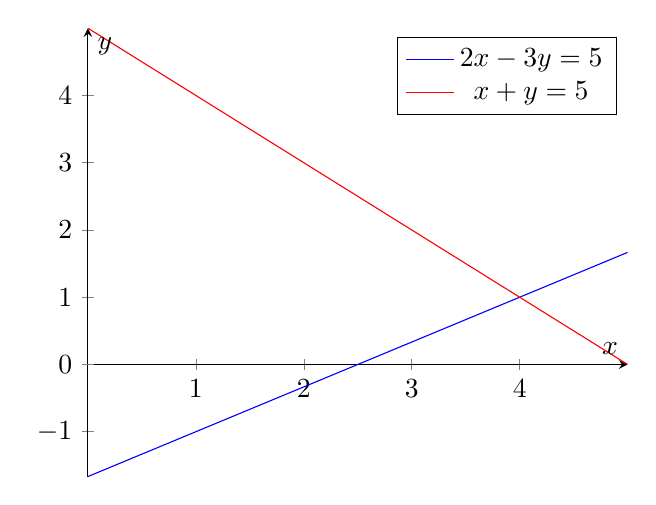
\begin{tikzpicture}
    \begin{axis}[axis lines=middle, xlabel={$x$}, ylabel={$y$}, xtick={0,1,2,3,4}, ytick={-1,1,2,3,4}, extra y ticks={0}]
    \addplot[domain=0:5, samples=100, color=blue]{(2*x-5)/3};
    \addplot[domain=0:5, samples=100, color=red]{5-x};
    \addlegendentry{$2x-3y=5$};
    \addlegendentry{$x+y=5$};
    \end{axis}
  \end{tikzpicture}
\end{fig}\n

Below is another example where the equations have no solution:\n

\begin{exm}
  The following is a system of linear equations with two unknowns:

  $$\begin{cases}
    2x-3y=-5\\
    2x-3y=0
  \end{cases}$$\s

   By plotting the two equations as two different straight lines on the same graph (see \rfig[\sctd{-1}]), where the green line is $2x-3y=5$ and the blue line is $2x-3y=0$, no solution can be found since they are parallel lines.
\end{exm}\n

\propdisp

\begin{fig}
  \centering
  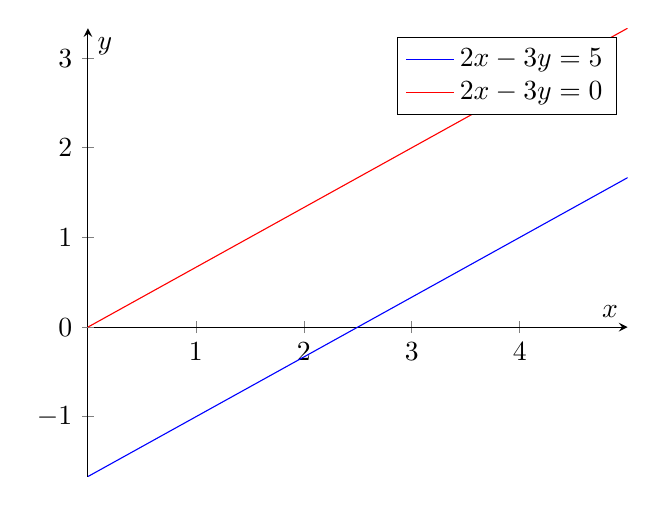
\begin{tikzpicture}
    \begin{axis}[axis lines=middle, xlabel={$x$}, ylabel={$y$}, xtick={0,1,2,3,4}, ytick={-1,1,2,3}, extra y ticks={0}]
    \addplot[domain=0:5, samples=100, color=blue]{(2*x-5)/3};
    \addplot[domain=0:5, samples=100, color=red]{2*x/3};
    \addlegendentry{$2x-3y=5$};
    \addlegendentry{$2x-3y=0$};
    \end{axis}
  \end{tikzpicture}
\end{fig}\n

Below is the third example where the equations have infinitely many solutions:\n

\begin{exm}
  The following is a system of linear equations with two unknowns:

  $$\begin{cases}
    2x-3y=-5\\
    2x-3y=-5
  \end{cases}$$\s

  In this case, the system has infinite solutions: for any real number $t$, $(t, \frac{2t+5}{3})$ is a solution. In a geometrical perspective, since the two lines coincide, their intersection is the whole line $2x-3y=-5$.
\end{exm}

\subsubsection{Intersections of Planes}
Different to systems of linear variables of two unknowns which can be represented in 2-dimensional space, systems of linear variables of three unknowns have to be represented in 3-dimensional space, and each of the equations are represented by a plane.\n

\begin{exm}
  The following is a system of linear equations with three unknowns:

  $$\begin{cases}
    2x+3y+3z=3\\
    2x-y=0
  \end{cases}$$\s

  The intersection of the two planes is a straight line, which can be expressed as

  $$\brc{\brr{\frac{3-3t}{8},\frac{3-3t}{4},t}\srm t\in\R}$$
\end{exm}\n

\begin{exm}
  The following is a system of linear equations with three unknowns:

  $$\begin{cases}
    2x+3y+3z=3\\
    2x+3y+3z=5\\
  \end{cases}$$\s

  Since the corresponding planes of the equations are parallel, the system has no solution.
\end{exm}\n

Suppose there are three equations with three variables that corresponds to three different planes. There are five types of solutions to this situation:

\begin{alist}
  \item All three planes are parallel to each other. The system has no solution.
  \item Two of the three planes are parallel to each other and the other plane does not. The system has solution of two straight lines.
  \item Intersection of any two planes is a straight line. The three lines from the intersection of planes are parallel to each other. The system has solution of three straight lines.
  \item The intersection of three planes is a straight line. The system has solution of one straight line.
  \item The intersection of three planes is a point. The system has a unique solution.
\end{alist}

\subsubsection{Addition of Vectors}
Beside from intersections of lines and planes, solving systems of equations with vectors is also a considerable choice.\n

\begin{exm}
  The following is a system of linear equations with two unknowns, written in a single vector form equation:

  $$x\begin{bmatrix}
    2\\
    1
  \end{bmatrix}+y\begin{bmatrix}
    -3\\
    1
  \end{bmatrix}=\begin{bmatrix}
    -5\\
    5
  \end{bmatrix}=b$$\s

  The problem now becomes finding the combination of the column vectors on the left side that produces the vector $b$ on the right side.
\end{exm}\n

Here are the system of linear equations used in examples in previous section:\n

\begin{exm}
  The following is a system of linear equations with two unknowns, written in a single vector form equation:

  $$x\begin{bmatrix}
    2\\
    2
  \end{bmatrix}+y\begin{bmatrix}
    -3\\
    -3
  \end{bmatrix}=\begin{bmatrix}
    -5\\
    0
  \end{bmatrix}$$\s

  $$x\begin{bmatrix}
    2\\
    2
  \end{bmatrix}+y\begin{bmatrix}
    -3\\
    -3
  \end{bmatrix}=\begin{bmatrix}
    -5\\
    -5
  \end{bmatrix}$$\s

  In both of the examples, the two vectors on the left side are colinear. For the first example, since the target vector is not colinear with the two vectors, there are no solutions for the system. For the second example, since the target vector is colinear with the two vectors, there are infinite solutions for the system.
\end{exm}\n

In fact, this method can also be applied to 3-dimensional cases:\n

\begin{exm}
  The following is a system of linear equations with three unknowns, written in a single vector form equation:

  $$x\begin{bmatrix}
    2\\
    4\\
    -2
  \end{bmatrix}+y\begin{bmatrix}
    1\\
    -6\\
    7
  \end{bmatrix}+z\begin{bmatrix}
    1\\
    0\\
    2
  \end{bmatrix}=\begin{bmatrix}
    5\\
    -2\\
    9
  \end{bmatrix}$$\s

  By finding the combination of column vectors on the left side, the solution set for the equation above is

  $$\begin{cases}
    x=1\\
    y=1\\
    z=2
   \end{cases}$$
\end{exm}\n

\begin{exm}
  In the following example, the three vectors are coplanar, which means they all lies on the same plane:

  $$x\begin{bmatrix}
    \frac{3}{2}\\
    -1\\
    0
  \end{bmatrix}+y\begin{bmatrix}
    0\\
    1\\
    -1
  \end{bmatrix}+z\begin{bmatrix}
    \frac{3}{2}\\
    0\\
    -1
  \end{bmatrix}=b$$\s

  Note that the three vectors lies on the plane $2x+3y+3z=0$. Similar to colinear cases in 2-dimensional space, the resulting vector $b$ determines number of solutions. For example, when

  $$b=b_{0}=\begin{bmatrix}
    0\\
    1\\
    1
  \end{bmatrix}$$\s

  the system has no solution, and when

  $$b=b_{\infty}=\begin{bmatrix}
    3\\
    -1\\
    -1
  \end{bmatrix}$$\s

  the system has infinite solutions.
\end{exm}

\propdisp

\subsection{Introduction to Systems of Linear Equations}
\subsubsection{Definition of Systems of Linear Equations}
\begin{dft}
  A \textbf{system of linear equations} is a collection of $m$ equations in the variable quantities $x_{1},x_{2},x_{3},\cdots,x_{n}$ of the form

  $$\begin{aligned}[t]
    a_{11}x_{1}+a_{12}x_{2}+a_{13}x_{3}+\cdots+a_{1n}x_{n}&=b_{1}\\
    a_{21}x_{1}+a_{22}x_{2}+a_{23}x_{3}+\cdots+a_{2n}x_{n}&=b_{2}\\
    &\vdots\\
    a_{m1}x_{1}+a_{m2}x_{2}+a_{m3}x_{3}+\cdots+a_{mn}x_{n}&=b_{m}
  \end{aligned}$$\s

  where the values of $a_{ij},b_{i}$ and $x_{j}$, $1<i<m,1<j<n$ are from the set of real numbers $\R$.
\end{dft}

\subsubsection{Possibilities of Solution Sets}
\begin{dft}
  A set $(s_{1},s_{2},\cdots,s_{n})$ is said to be a \textbf{solution} of a system of linear equations in $n$ variables if every equation in the system is valid after substitution. The \textbf{solution set} of a linear equation is the combination of all solutions of the system of linear equations.
\end{dft}\n

\begin{exm}
  The following is a system of linear equations:

  $$\begin{aligned}[t]
    x_{1}+2x_{2}+x_{4}&=7\\
    x_{1}+x_{2}+x_{3}-x_{4}&=3\\
    3x_{1}+x_{2}+5x_{3}-7x_{4}&=1
  \end{aligned}$$\s

  and it can be rewritten as

  $$\begin{aligned}[t]
    1x_{1}+2x_{2}+0x_{3}+1x_{4}&=7\\
    1x_{1}+1x_{2}+1x_{3}-1x_{4}&=3\\
    3x_{1}+1x_{2}+5x_{3}-7x_{4}&=1
  \end{aligned}$$\s

  Note that the system has infinitely many solutions, and the solution set is

  $$\left\{ (-1-2a+3b,4+a-2b,a,b)\mid a,b\;\text{real numbers}\right\}$$
\end{exm}\n

Here the theorem about the possibilities of solution sets is introduced:\n

\begin{thm}
  Any system of linear equations with real numbers as coefficients can have a unique solution, infinite solutions or no solution.
\end{thm}\n

Therefore it is impossible for a system of linear equations to have exactly two solutions, for example. Also note that the above theorem is only true when the coefficients are real numbers. In higher mathematics, coefficients can also be finite fields which will affect numbers of solutions.

\subsubsection{Equivalent Systems and Equation Operations}
\begin{dft}
  Two systems of linear equations are said to be \textbf{equivalent} if their solution sets are equal, and the two systems are said to be \textbf{equivalent systems}.
\end{dft}\n

\begin{dft}
  Given a system of linear equations, the following three operations will transform a system into another one:

  \begin{alist}
    \item Swap the position of any two equations in the list of equations.
    \item Perform a non-zero scalar multiplication to an equation in the list of equations.
    \item Perform a scalar multiplication to an equation, and then add to another equation on both sides of the equality.
  \end{alist}

  The above operations are all called \textbf{equation operations}.
\end{dft}\n

Note that the following theorem about equivalent systems and equation operations is true:\n

\begin{pst}
  If the transformed system is created by applying any one of three equation operations to an original system of linear equations, then the original system and the transformed system are equivalent.
\end{pst}

\pagebreak

\section{Linear Algebra with Matrices}
\subsection{Introduction to Matrices}
\subsubsection{Matrix and Vector Notations}
In order to solve systems of linear equations systematically, a useful and powerful tool called matrix is used.\n

\begin{dft}
  A $m\times n$ \textbf{matrix} is a rectangular layout of numbers having $m$ rows and $n$ columns. The matrix is bracketed with either parentheses or brackets. Rows are counted from top to bottom and columns are counted from left to right, and for a matrix $A$, the notation $[A]_{ij}$ refers to the number in row $i$ and column $j$ of the matrix $A$.
\end{dft}\n

\begin{exm}
  The following is a matrix

  $$B=\begin{bmatrix}
  1 & 0 & 2 & 5\\
  3 & -2 & -7 & 4\\
  -1 & 4 & 6 & -3
  \end{bmatrix}$$\s

  with $m=3$ rows and $n=4$ columns. Note that $[B]_{2,3}=-7$ and $[B]_{3,4}=-3$.
\end{exm}\n

In fact, during the solving process of systems of linear equations, the names of the variables do not matter at all. On the other hand, using matrix notations can describe linear systems, solve the systems and describe the solution sets with much ease.\n

\begin{dft}
  A \textbf{column vector} of size $m$ is an ordered list of $m$ numbers in a vertical order from top to bottom.
\end{dft}\n

At times, a column vector is also simply called a vector. Commonly, the notation of a vector is usually small letters in bold ($\mathbf{v}$) or with arrows on top of the symbol ($\vec{v}$). The entry of vector $\mathbf{v}$ in location $i$ is in notation $[\mathbf{v}]_{i}$.\n

\begin{dft}
  The \textbf{zero vector} of size $m$ is the column vector of size $m$ with each entry is zero:

  $$\mathbf{0}=\begin{bmatrix}
  0\\
  0\\
  \vdots\\
  0
  \end{bmatrix}$$\s

  or in entry notations, $[\mathbf{0}]_{i}=0$ for $1\leq i\leq m$.
\end{dft}

\propdisp

\subsubsection{Partitions of Matrices}
\begin{dft}
  A \textbf{partition} of a matrix is a horizontal or vertical line dividing the matrix into different areas. A matrix is the same with or without partitions, but partitions can provide better reading if required.
\end{dft}\n

\begin{exm}
  Suppose $A$ is a matrix and $\mathbf{u}$ is a column vector where

  $$A=\begin{bmatrix}
    1 & 2\\
    3 & 4\\
  \end{bmatrix},\mathbf{u}=\begin{bmatrix}
    5\\
    6
  \end{bmatrix}$$

  Then

  $$[A\!\mid\!\mathbf{u}]=\left[ \begin{array}{@{}cc|c@{}}
    1 & 2 & 5\\
    3 & 4 & 6
  \end{array}\right]$$
\end{exm}

\subsubsection{Matrix Representations of Linear Systems}
\begin{dft}
  For a system of linear eqautions

  $$\begin{aligned}[t]
    a_{11}x_{1}+a_{12}x_{2}+a_{13}x_{3}+\cdots+a_{1n}x_{n}&=b_{1}\\
    a_{21}x_{1}+a_{22}x_{2}+a_{23}x_{3}+\cdots+a_{2n}x_{n}&=b_{2}\\
    &\vdots\\
    a_{m1}x_{1}+a_{m2}x_{2}+a_{m3}x_{3}+\cdots+a_{mn}x_{n}&=b_{m}
  \end{aligned}$$\s

  the \textbf{coefficient matrix} is the $m\times n$ matrix

  $$A=\begin{bmatrix}
    a_{11} & a_{12} & a_{13} & \cdots & a_{1n}\\
    a_{21} & a_{22} & a_{23} & \cdots & a_{2n}\\
    \vdots & \vdots & \vdots & \ddots & \vdots\\
    a_{m1} & a_{m2} & a_{m3} & \cdots & a_{mn}
  \end{bmatrix}$$\s

  the \textbf{vector of constants} is the column vector of size $m$

  $$\mathbf{b}=\begin{bmatrix}
    b_{1}\\
    b_{2}\\
    \vdots\\
    b_{m}
  \end{bmatrix}$$\s

  and the \textbf{solution vector} is the column vector of size $n$

  $$\mathbf{x}=\begin{bmatrix}
    x_{1}\\
    x_{2}\\
    \vdots\\
    x_{n}
  \end{bmatrix}$$
\end{dft}\n

\begin{dft}
  If $A$ is the coefficient matrix of a system of linear equations and $b$ is the vector of constants, then $\mathit{LS}(A,\mathbf{b})$ is the shorthand expression for the system of linear equations, which is referred as the \textbf{matrix representation} of the linear system. Also, the \textbf{augmented matrix} of the linear system $[A\!\mid\!\mathbf{b}]$ is the $m\times(n+1)$ matrix with matrix $A$ on the left and column vector $\mathbf{b}$ on the right.
\end{dft}

% edit here

\subsubsection{Row Operations}
An augmented matrix can represent the system of linear equations, which can also perform row operations as before. Recall the three equation operations:

\begin{alist}
  \item Swap the position of any two equations in the list of equations.
  \item Perform a non-zero scalar multiplication to an equation in the list of equations.
  \item Perform a scalar multiplication to an equation, and then add to another equation on both sides of the equality.
\end{alist}

For augmented matrices, the following operations works similarly as the equation opertions above, but to transform matrices into another one with the same size:

\begin{alist}
  \item Swap any two rows in a matrix.
  \item Perform a non-zero scalar multiplication to every entry of a row in a matrix.
  \item Perform a scalar multiplication to every entry of a row in a matrix, and then add to another row in the same columns. The first row will remain unchanged while the second row is replaced by new values.
\end{alist}

The three operations above are called \textbf{row operations}. There are symbolic shorthands to describe these row operations:

\begin{alist}
  \item $R_{i}\leftrightarrow R_{j}$ : Swap row $i$ and row $j$.
  \item $\alpha R_{i}$ : Multiply row $i$ by the non-zero scalar $\alpha$.
  \item $\alpha R_{i}+R_{j}$ : Multiply row $i$ by the scalar $\alpha$ and add to row $j$.
\end{alist}

Suppose there are two matrices $A$ and $B$ of the same size. $A$ and $B$ are said to be \textbf{row-equivalent} if one can be obtained from the other by a sequence of row operations. Note that all row operations are reversible, so the distinction between $A$ is row-equivalent to $B$ and $B$ is row-equivalent to $A$ does not matter. With this definition, the following theorem applies:\n

\begin{pst}
  Suppose $A$ and $B$ are row-equivalent augmented matrices, then the systems of linear equations that the two matrices represent are equivalent systems.
\end{pst}

\subsection{Matrix Operations}
\subsubsection{Matrix Equality, Addition and Scalar Multiplication}
\begin{dft}
  Recall $M_{mn}$ is the set of $m\times n$ matrices with real entries. Suppose there are two matrices $A$ and $B$ with size $m\times n$. The following definitions can be applied:\n

  \begin{alist}
    \item The two matrices $A$ and $B$ are said to be \textbf{equal}, written as $A=B$ if

    $$[A]_{ij}=[B]_{ij}\;\;\;\;\text{for all}1\leq i\leq m,1\leq j\leq n$$

    \item The \textbf{sum} of two matrices $A$ and $B$, written as $A+B$, is a matrix with size $m\times n$ where

    $$[A+B]_{ij}=[A]_{ij}+[B]_{ij}\;\;\;\;\text{for all}1\leq i\leq m,1\leq j\leq n$$

    \item The \textbf{scalar multiple} of the matrix $A$ by $\alpha$, where $\alpha\in\R$, is a matrix with size $m\times n$, written as $\alpha A$ where

    $$[\alpha A]_{ij}=\alpha[A]_{ij}\;\;\;\;\text{for all}1\leq i\leq m,1\leq j\leq n$$

    \item The $m\times n$ \textbf{zero matrix} is written as $O=O_{m\times n}$ and defined by $[O]_{ij}=0$ for all $1\leq i\leq m,1\leq j\leq n$.

    \item The \textbf{addictive inverse} of the matrix $A$, written as $-A$, is defined by $-A=(-1)A$.
  \end{alist}
\end{dft}\n

\begin{pst}
  Below are some properties satisfied by addition and scalar multiplication:

  \begin{alist}
    \item \textbf{Commutativity, Matrices}\\
    If $A,B\in M_{mn}$, then $A+B=B+A$.

    \item \textbf{Addictive Associativity, Matrices}\\
    If $A,B,C\in M_{mn}$, then $A+(B+C)=(A+B)+C$.

    \item \textbf{Zero Matrix, Matrices}\\
    $A+O=A$ for all $A\in M_{mn}$.

    \item \textbf{Addictive Inverse, Matrices}\\
    $A+(-A)=O$ for all $A\in M_{mn}$.

    \item \textbf{Scalar Multiplication Associativity, Matrices}\\
    If $\alpha,\beta\in\R$ and $A\in M_{mn}$, then $\alpha(\beta A)=(\alpha\beta)A$.

    \item \textbf{Distributivity across Matrix Addition, Matrices}\\
    If $\alpha\in\R$ and $A,B\in M_{mn}$, then $\alpha(A+B)=\alpha A+\alpha B$.

    \item \textbf{Distributivity across Scalar Addition, Matrices}\\
    If $\alpha,\beta\in\R$ and $A\in M_{mn}$, then $(\alpha+\beta)A=\alpha A+\beta A$.

    \item \textbf{One, Matrices}\\
    If $A\in M_{mn}$, then $1A=A$.
  \end{alist}
\end{pst}

\subsubsection{Transposes and Symmetric Matrices}
Suppose there is a matrix $A$ of size $m\times n$. The \textbf{transpose} of the matrix $A$ is the matrix $A^{t}$ of size $n\times m$ where

$$[A^{t}]_{ij}=[A]_{ji}\;\;\;\;\text{for all }1\leq i\leq n,1\leq j\leq m$$\s

With the definition of transposes of matrices, a matrix $A$ is said to be \textbf{symmetric} if $A=A^{t}$. Note that the following theorem is always applicable to symmetric matrices:\n

\begin{pst}
  Suppose $A$ is a symmetric matrix, then $A$ is also a square matrix.\n

  \prf Suppose $A$ is a $n\times m$ matrix. Then $A^{t}$ is a $m\times n$ matrix. In order for $A$ and $A^{t}$ to be equal, they must be in the same dimension. Hence $m=n$ and $A$ is a square matrix.
\end{pst}\n

The following are three theorems that are easy to prove matrix equalities with learnt notations and techniques:\n

\begin{pst}
  Suppose $A$ and $B$ are $m\times n$ matrices, then $(A+B)^{t}=A^{t}+B^{t}$.\n

  \prf For $1\leq i\leq n,1\leq j\leq m$,

  $$\begin{aligned}[t]
    [(A+B)^{t}]_{ij}&=[(A+B)]_{ji}\\
    &=[A]_{ji}+[B]_{ji}\\
    &=[A^{t}]_{ij}+[B^{t}]_{ij}\\
    &=[A^{t}+B^{t}]_{ij}
  \end{aligned}$$\s

  Since every entry of the matrices $(A+B)^{t}$ and $A^{t}+B^{t}$ agrees, the matrices are equal.
\end{pst}\n

\begin{pst}
  Suppose $\alpha\in\R$ and $A$ is an $m\times n$ matrix, then $(\alpha A)^{t}=\alpha A^{t}$.\n

  \prf For $1\leq i\leq n,1\leq j\leq m$,

  $$\begin{aligned}[t]
    [(\alpha A)^{t}]_{ji}&=[\alpha A]_{ij}\\
    &=\alpha[A]_{ij}\\
    &=\alpha[A^{t}]_{ji}\\
    &=[\alpha A^{t}]_{ji}
  \end{aligned}$$\s

  Since every entry of the matrices $(\alpha A)^{t}$ and $\alpha A^{t}$ agrees, the matrices are equal.
\end{pst}\n

\begin{pst}
  Suppose $A$ is an $m\times n$ matrix, then $(A^{t})^{t}=A$.\n

  \prf For $1\leq i\leq m,1\leq j\leq n$,

  $$\begin{aligned}[t]
    [(A^{t})^{t}]_{ij}&=[A^{t}]_{ji}\\
    &=[A]_{ij}
  \end{aligned}$$\s

  Since every entry of the matrices $(A^{t})^{t}$ and $A$ agrees, the matrices are equal.
\end{pst}\n

\subsection{Matrix Multiplication}
\subsubsection{Matrix-Vector Product}
\begin{dft}
  Suppose that $A$ is an $m\times n$ matrix with columns $A_{1},A_{2},\cdots,A_{n}$ and $\mathbf{u}$ is a vector of size $n$, then the \textbf{matrix-vector product} of $A$ with $\textbf{u}$ is the linear combination

  $$A\mathbf{u}=[\mathbf{u}]_{1}A_{1}+[\mathbf{u}]_{2}A_{2}+\cdots+[\mathbf{u}]_{n}A_{n}$$
\end{dft}\n

As shown above, the matrix-vector product is yet another version of multiplication. Note that an $m\times n$ matrix multiplies with a vector of size $n$ will produce a vector of size $m$.\n

With the definition of matrix-vector product, systems of linear equations can be represented compactly with a matrix-vector product and column vector equality. This yields a very popular alternative to the unconventional $LS(A,\mathbf{b})$ notation.\n

\begin{pst}
  The set of solutions to the linear system $LS(A,\mathbf{b})$ equals the set of solutions for $x$ in the vector equation $A\mathbf{x}=\mathbf{b}$.\n

  \prf $$\begin{aligned}[t]
    &\mathbf{x}\text{ is a solution to }LS(A,\mathbf{b})\\
    &\Leftrightarrow[\mathbf{x}]_{1}A_{1}+[\mathbf{x}]_{2}A_{2}+[\mathbf{x}]_{n}A_{n}=b\\
    &\Leftrightarrow\mathbf{x}\text{ is a solution to }A\mathbf{x}=\mathbf{b}
  \end{aligned}$$
\end{pst}\n

\begin{pst}
  Suppose $A$ and $B$ are $m\times n$ matrices such that $A\mathbf{x}=B\mathbf{x}$ for any $\mathbf{x}\in\R^{n}$, then $A=B$.
\end{pst}\n

\subsubsection{Introduction to Matrix Multiplication}
With the method of matrix-vector product, such method can also apply to multiplication of two matrices. Suppose $A$ is an $m\times n$ matrix and $B$ is an $n\times p$ matrix with columns $B_{1},B_{2},\cdots,B_{p}$, then the matrix product of $A$ and $B$ is the $m\times p$ matrix where

$$AB=A[B_{1}\!\mid\!B_{2}\!\mid\!\cdots\!\mid\!B_{p}]=[AB_{1}\!\mid\!AB_{2}\!\mid\!\cdots\!\mid\!AB_{p}]$$\s

Notice that the matrix product $BA$ does not exist due to inappropriate size of the two matrices. Even if the size allows the matrix product to exist, the matrix product will not be the same as the other matrix product. This is because many of the ideas about multiplication will not apply to matrix multiplication. In this case, matrix multiplication is not commutative, which means that the order matters.\n

\begin{pst}
  Suppose $A$ is an $m\times n$ matrix and $B$ is an $n\times p$ matrix, then for $1\leq i\leq m, 1\leq j\leq p$, the individual entries of $AB$ is given by

  $$\begin{aligned}[t]
    [AB]_{ij}&=[A]_{i1}[B]_{1j}+[A]_{i2}[B]_{2j}+\cdots+[A]_{in}[B]_{nj}\\
    &=\sum_{k=1}^{n}[A]_{ik}[B]_{kj}
  \end{aligned}$$
\end{pst}\n

In fact, this is often used as the definition of the matrix product $AB$.

\subsubsection{Properties of Matrix Multiplication}
\begin{pst}
  Suppose $A$ is an $m\times n$ matrix, then the following equalities apply:
  \begin{alist}
    \item $AO_{n\times p}=A_{m\times p}$
    \item $O_{p\times m}A=O_{p\times n}$
  \end{alist}
\end{pst}\n

\begin{pst}
  Suppose $A$ is an $m\times n$ matrix, then the following equalities apply:
  \begin{alist}
    \item $AI_{n}=A$
    \item $I_{m}A=A$
  \end{alist}
\end{pst}\n

Note that the matrix $I$ is given the name of identity matrix since it behaves with matrix multiplication like the scalar $1$ does in scalar multiplication, as shown in the previous theorem. Multiplying by the identity matrix is to have no effect on the other matrix.\n

\begin{pst}
  Suppose $A$ is an $m\times n$ matrix, $B$ and $C$ are $n\times p$ matrices, and $D$ is a $p\times s$ matrix, then the following equalities apply:
  \begin{alist}
    \item $A(B+C)=AB+AC$
    \item $(B+C)D=BD+CD$
  \end{alist}
\end{pst}\n

\begin{pst}
  Suppose $A$ is an $m\times n$ matrix, $B$ is an $n\times p$ matrix and $\alpha$ is a scalar, then $\alpha(AB)=(\alpha A)B=A(\alpha B)$.
\end{pst}\n

\begin{pst}
  Suppose $A$ is an $m\times n$ matrix, $B$ is an $n\times p$ matrix and $D$ is a $p\times s$ matrix, then $(AB)D=A(BD)$.
\end{pst}\n

\begin{pst}
  Suppose $A$ is an $m\times n$ matrix and $B$ is an $n\times p$ matrix, then $(AB)^{t}=B^{t}A^{t}$.
\end{pst}

\subsubsection{Row Operations and Matrix Multiplication}
Recall the elementary row operations:

\begin{alist}
  \item Swap any two rows in a matrix.
  \item Perform a non-zero scalar multiplication to every entry of a row in a matrix.
  \item Perform a scalar multiplication to every entry of a row in a matrix, and then add to another row in the same columns. The first row will remain unchanged while the second row is replaced by new values.
\end{alist}

\begin{pst}
  Let matrix $A\in M_{mn}$, $B$ be a matrix obtained by applying one of the row operations on $A$, and $J$ be a matrix obtained by applying the exact same row operation on $I_{m}$, then $JA=B$.
\end{pst}

\subsection{Reduced Row Echelon Form}
\subsubsection{Introduction to Reduced Row Echelon Form}
Here are some terminology before introducing reduced row echelon form:\n

\begin{dft}
  \begin{alist}
    \item A \textbf{zero row} is a row consists of only $0$.
    \item The \textbf{leftmost entry} of a row is the first nonzero entry of a row.
    \item The \textbf{index} of the leftmost entry of a row is the index of the first nonzero entry, denoted by $l_{i}$ for row $i$.
  \end{alist}
\end{dft}\n

\begin{exm}
  The following is a matrix

  $$A=\begin{bmatrix}
  0 & 1 & 0 & 1 & 2\\
  0 & 0 & 0 & 3 & 0\\
  0 & 0 & 1 & 0 & 1\\
  0 & 0 & 0 & 0 & 0
  \end{bmatrix}$$\s

  Note that the index of leftmost entry of row $1$ is $l_{1}=2$, that of row $2$ is $l_{2}=4$ and that of row $3$ is $l_{3}=3$. Row $4$ is a zero row.
\end{exm}\n

\begin{dft}
  A matrix is said to be in \textbf{reduced row echelon form}, RREF in short, if it meets all of the conditions below:

  \begin{alist}
    \item If there is a row where every entry is zero, then this row lies below any other row with nonzero entries.
    \item The leftmost nonzero entry of a row is equal to $1$.
    \item The leftmost nonzero entry of a row is the only nonzero entry in its column.
    \item If $i<j$ and both row $i$ and row $j$ are not zero rows, then $l_{i}<l_{j}$.
  \end{alist}
\end{dft}\n

With the definition of reduced row echelon form above, there are more definition based on reduced row echelon form:\n

\begin{dft}
  \begin{alist}
    \item A row of only entries of $0$ is a zero row, and the leftmost nonzero entry of a nonzero row is a \textbf{leading 1}.
    \item A column that contains a leading 1 is called a \textbf{pivot column}, denoted by $D=\left\{ d_{1},d_{2},\cdots,d_{r}\right\}$ where in ascending order.
    \item Columns that are not pivot columns are denoted by $F=\left\{ f_{1},f_{2},\cdots,f_{n-r}\right\}$ where in ascending order.
  \end{alist}
\end{dft}\n

Note that the number of nonzero rows is denoted by $r$ as above, and it should always equal to the number of leading 1's and number of pivot columns.

\subsubsection{Transforming Matrices to Reduced Row Echelon Form}
Below is a theorem that states that any matrix can be transformed to reduced row echelon form:\n

\begin{thm}
  Suppose $A$ is a matrix, then there exists a matrix $B$ such that

  \begin{alist}
    \item $A$ and $B$ are row-equivalent.
    \item $B$ is in reduced row echelon form.
  \end{alist}
\end{thm}\n

With the theorem above, suppose $A$ has $m$ rows and $n$ columns. There is always a process to convert $A$ into $B$ via row operations. Such procedure is known as \textbf{Gaussian elimination} or \textbf{Gauss-Jordan elimination}. The following is an example of the procedure mentioned:\n

\begin{exm}
  The following is a matrix

  $$A=\begin{bmatrix}
  0 & 0 & 1 & 1 & 4\\
  0 & 0 & 1 & 1 & 3\\
  1 & 1 & 2 & 4 & 8\\
  2 & 2 & 5 & 9 & 19\\
  \end{bmatrix}$$\s

  Consider the first row, note that the first entry of the row is $0$, therefore consider the first column. If the first entry of the row is nonzero, this step can be skipped. The third entry of the column is a nonzero entry, hence perform $R_{1}\leftrightarrow R_{3}$:

  $$\xrightarrow[ ]{R_{1}\leftrightarrow R_{3}}\begin{bmatrix}
  1 & 1 & 2 & 4 & 8\\
  0 & 0 & 1 & 1 & 3\\
  0 & 0 & 1 & 1 & 4\\
  2 & 2 & 5 & 9 & 19\\
  \end{bmatrix}$$\s

  Note that the fourth entry of the column is also a nonzero entry, but in this case choosing an entry that is equal to $1$ or $-1$ will make future steps easier. Now check the leftmost entry of the first row, and peform $\frac{1}{a}R_{1}$ where $a$ is the entry. This step is skipped in this example since the leftmost entry of the first row is already $1$.\n

  Now eliminate the remaining nonzero entries within the same column. In this example, the fourth entry of the column is nonzero, thus perform $-2R_{1}+R_{4}$:

  $$\xrightarrow[ ]{-2R_{1}+R_{4}}\begin{bmatrix}
  1 & 1 & 2 & 4 & 8\\
  0 & 0 & 1 & 1 & 3\\
  0 & 0 & 1 & 1 & 4\\
  0 & 0 & 1 & 1 & 3\\
  \end{bmatrix}$$\s

  The first row and first column is completed and can be ignored:

  $$\begin{bmatrix}
  * & * & * & * & *\\
  * & 0 & 1 & 1 & 3\\
  * & 0 & 1 & 1 & 4\\
  * & 0 & 1 & 1 & 3\\
  \end{bmatrix}$$\s

  Note that the first leftmost entry of the row is at row $2$ and column $3$, so consider the third column and perform elimination, including the ignored row $1$:

  $$\xrightarrow[ ]{-2R_{2}+R_{1},-R_{2}+R_{3},-R_{2}+R_{4}}\begin{bmatrix}
  1 & 1 & 0 & 2 & 2\\
  0 & 0 & 1 & 1 & 3\\
  0 & 0 & 0 & 0 & 1\\
  0 & 0 & 0 & 0 & 0\\
  \end{bmatrix}$$\s

  Repeat the process:

  $$\begin{bmatrix}
  * & * & * & * & *\\
  * & * & * & * & *\\
  * & * & * & 0 & 1\\
  * & * & * & 0 & 0\\
  \end{bmatrix}$$\s

  $$\xrightarrow[ ]{-2R_{3}+R_{1},-3R_{3}+R_{2}}\begin{bmatrix}
  1 & 1 & 0 & 2 & 0\\
  0 & 0 & 1 & 1 & 0\\
  0 & 0 & 0 & 0 & 1\\
  0 & 0 & 0 & 0 & 0\\
  \end{bmatrix}$$\s

  until the matrix is in reduced row echelon form.
\end{exm}

\subsubsection{Uniqueness of Reduced Row Echelon Form}
\begin{thm}
  Suppose $A$ is an $m\times n$ matrix, and $B$ and $C$ are$m\times n$ matrix that are row-equivalent to $A$ and in reduced row echelon form, then $B=C$.
\end{thm}\n

With the above theorem, we can solve systems of equations in matrix form by reduced row echelon form.

\subsection{Types of Solution Sets}
\subsubsection{Consistent Systems}
With the reduced row echelon form, augmented matrices of systems of linear equations can be analyzed more systematically and carefully. In this section, the fact that every system of linear equations has either zero, one or infinitely many solutions will be proven in detail, thus routinely solve any linear system.\n

\begin{dft}
  A system is said to be \textbf{consistent} if it has at least one solution. A system with no solution is \textbf{inconsistent}.
\end{dft}\n

\subsubsection{Free and Dependent Variables}
Recall the following terms about reduced row echelon form:\n

\begin{dft}
  Let $A$ be a matrix in reduced row echelon form.
  \begin{alist}
    \item The number of nonzero rows is called the \textbf{rank} of $A$ and is denoted by $r$.
    \item The set of the column indexes for the pivot columns is denoted by

    $$D=\left\{ (d_{1},d_{2},\cdots,d_{r})\mid d_{1}<d_{2}<\cdots<d_{r}\right\}$$

    \item The set of the column indexes that are not pivot columns is denoted by

    $$D=\left\{ (f_{1},f_{2},\cdots,f_{n-r})\mid f_{1}<f_{2}<\cdots<f_{n-r}\right\}$$
  \end{alist}
\end{dft}\n

With the definition above, free and dependent variables can also be defined as follows:\n

\begin{dft}
  Suppose $A$ is the augmented matrix of a consistent system of linear equations and $B$ is a row-equivalent matrix in reduced row echelon form. If $j$ is the index of a pivot column of $B$, then the variable $x_{j}$ is \textbf{dependent}. A variable that is not dependent is \textbf{independent} or \textbf{free}.
\end{dft}\n

\begin{thm}
  Suppose the matrix $A$ is the augmented matrix of a system of linear equations with $n$ variables, and $B$ is a row-equivalent matrix in reduced row echelon form with $r$ nonzero rows, then the following is true:

  \begin{alist}
    \item The system of equations is inconsistent if and only if column $n+1$ (i.e. the last column) of $B$ is a pivot column.
    \item The system of equations is also inconsistent if and only if the last nonzero row is $(0,0,\cdots,0,1)$.
    \item Equivalently a system is consistent if and only if column $n+1$ is not a pivot column of $B$.
  \end{alist}
\end{thm}

\subsubsection{Interpretations of Reduced Row Echelon Form}
\begin{thm}
  Suppose $A$ is the augmented matrix of a consistent system of linear equations with $n$ variables, and $B$ is a row-equivalent matrix in reduced row echelon form with $r$ pivot columns. Then $r\leq n$. If $r=n$, then the system has unique solution, and if $r<n$, then the system has infinitely many solutions.\n

  \prf Notice that $B$ has $n+1$ columns, so there can be at most $n+1$ pivot columns, i.e. $r\leq n+1$. If $r=n+1$, then every column in $B$ is pivot column, in particular, the last column is also a pivot column. However, the previous theorem tells us that the system is inconsistent, which is contrary to the hypothesis. Then $r\leq n$.\n

  When $r=n$, then there are $n-r=0$ free variables, and the solution is unique. On the other hand, when $r<n$, there are $n-r>0$ free variables, and these free variables can be adjusted to create infinitely many solutions.
\end{thm}\n

The next theorem simply states a conclusion from the previous proof, in order to state explicitly the number of free variables in a consistent system.\n

\begin{thm}
  Suppose $A$ is the augmented matrix of a consistent system of linear equations with $n$ variables, and $B$ is a row-equivalent matrix in reduced row echelon form with $r$ nonzero rows, then the solution set can be described with $n-r$ free variables.
\end{thm}\n

With the number of free variables, possible solution sets for linear systems can be easily found, by the following theorem:\n

\begin{thm}
  A system of linear equations has no solutions, a unique solution or infinitely many solutions.\n

  \prf If the system is inconsistent, then the system has no solutions. Now suppose the system is consistent, if it has no free variables, then it has a unique solution. Otherwise, it has infinitely many solutions.
\end{thm}

\begin{thm}
  Suppose a consistent system of linear equations has $m$ equations in $n$ variables, then if $n>m$, then the system has infinitely many solutions.\n

  \prf Suppose there is an augmented matrix of system of linear equations that is row-equivalent to a matrix in reduced row echelon form with $r$ nonzero rows. Since the original matrix has $m$ rows in total, the number of nonzero rows should be less than or equal to $m$, which is $r\leq m$. Note that the number of free variables

  $$n-r\geq n-m>0$$

  based on the hypothesis $n>m$. A consistent system with free variables will then have infinitely many solutions, according to {\color{zr}\textit{Theorem 2.36}}.
\end{thm}

\subsection{Homogeneous Systems of Equations}
\subsubsection{Definition of Homogeneous Systems}
\begin{dft}
  A system of linear equations $LS(A,\mathbf{b})$ is \textbf{homogeneous} if the vector of constants is the zero vector, or in other words, $\mathbf{b}=\mathbf{0}$. The \textbf{homogeneous system} of $LS(A,\mathbf{b})$ can be expressed as $LS(A,\mathbf{0})$.
\end{dft}\n

Note that homogeneous systems have an identical property:\n

\begin{pst}
  Suppose a system of linear equation is homogeneous, then the system is consistent.\n

  \prf By setting every variable to $0$, the left hand side of all equations will equal to $0$, so does the right hand side.
\end{pst}

\subsubsection{Solutions of Homogeneous Systems}
With the above theorem, the definition of trivial solution is introduced:\n

\begin{dft}
  It is always possible to put the zero vector $\mathbf{0}$ into any homogeneous system as a solution. Such a solution is called a \textbf{trivial solution}.
\end{dft}\n

\begin{thm}
  Suppose a homogeneous system of linear equations has $m$ equations in $n$ variables with $n>m$, then the system has infinitely many solutions.\n

  \prf By {\color{zr}\textit{Proposition 2.41}}, the system is consistent, along with {\color{zr}\textit{Theorem 2.39}}, the system has infinitely many solutions.
\end{thm}

\subsubsection{Null Space of Matrices}
\begin{dft}
  The \textbf{null space} of a matrix $A$, denoted by $N(A)$, is the set of all vectors that are solutions to the homogeneous system $LS(A,\mathbf{0})$.
\end{dft}\n

\begin{exm}
  The following is a matrix

  $$A=\begin{bmatrix}
  1 & 4 & 0 & -1 & 0 & 7 & -9\\
  2 & 8 & -1 & 3 & 9 & -13 & 7\\
  0 & 0 & 2 & -3 & -4 & 12 & -8\\
  -1 & -4 & 2 & 4 & 8 & -31 & 37\\
  \end{bmatrix}$$\s

  Note that

  $$\mathbf{x}=\begin{bmatrix}
  3\\
  0\\
  -5\\
  -6\\
  0\\
  0\\
  1
\end{bmatrix},\;\mathbf{y}=\begin{bmatrix}
  -4\\
  1\\
  -3\\
  -2\\
  1\\
  1\\
  1
  \end{bmatrix}$$\s

  are both in $N(A)$ since $A\mathbf{x}=\mathbf{0}$ and $A\mathbf{y}=\mathbf{0}$.
\end{exm}

\subsubsection{Augmented Matrices and Coefficient Matrices}
The augmented matrix for the homogeneous system of linear equaations $LS(A,\mathbf{0})$ is $[A\!\mid\!\mathbf{0}]$. Note that any row operations will not have any effect on the last zero column. If

$$A\xrightarrow[ ]{\text{row operations}}B$$\s

then

$$[A\!\mid\!\mathbf{0}]\xrightarrow[ ]{\text{same row operations}}[B\!\mid\!\mathbf{0}]$$

\subsubsection{Nonsingular Matrices}
In this section it is specialized that only matrices that have equal number of rows and columns, or in other words, systems with equal number of equations and variables are considered.\n

\begin{dft}
  A matrix with $m$ rows and $n$ columns is a \textbf{square matrix} if $m=n$. In such a case, the matrix is said to have \textbf{size} $n$. In order to emphasize the situation where the matrix is not square, such a matrix can be said as a \textbf{rectangular matrix}.
\end{dft}\n

\begin{dft}
  Suppose matrix $A$ is a square matrix, and the solution set to the homogeneous linear system of equations $LS(A,\mathbf{0})$ is $\left\{ \mathbf{0}\right\}$, or in other words, it has only the trivial solution, then $A$ is a \textbf{nonsingular matrix}. Otherwise, $A$ is a \textbf{singular matrix}.
\end{dft}\n

Also recall the identity matrix, with the definition of square matrices:\n

\begin{dft}
  The \textbf{identity matrix} with size $m$, $I_{m}$, is defined by

  $$[I_{m}]_{ij}=\begin{cases}
    1,\; i=j\\
    0,\; i\neq j
   \end{cases}\;\;\;\; 1\leq i,j\leq m$$
\end{dft}\n

Note that every identity matrix is square, in reduced row echelon form, and every column is a unique pivot column.\n

\begin{thm}
  Suppose $A$ is a square matrix and $B$ is a row-equivalent matrix in reduced row echelon form, then $A$ is nonsingular if and only if $B$ is the identity matrix.\n

  \prf {\color{zr}$\mathit{(\Leftarrow)}$} Suppose $B$ is the identity matrix. When the augmented matrix $[A\!\mid\!\mathbf{0}]$ is reduced, the result is $[B\!\mid\!\mathbf{0}]=[I_{m}\!\mid\!\mathbf{0}]$. The number of nonzero rows is equal to the number of eqautions in the linear system of eqautions $LS(A,\mathbf{0})$, so it has no free variables. Then the homogeneous system $LS(A,\mathbf{0})$ has only one unique solution, which is the trivial solution.\n

  {\color{zr}$\mathit{(\Rightarrow)}$} If $A$ is nonsingular, then the homogeneous system $LS(A,\mathbf{0})$ has only unique solution, which means there are no free variables in the description of the solution set. By {\color{zr}\textit{Theorem 2.37}}, the system has $n-r$ free variables, in which $n=r$ in this case. Thus $B$ has $n$ pivot columns among its $n$ columns, forcing $B$ to be the identity matrix.
\end{thm}

\subsubsection{Null Space of Nonsingular Matrices}
Below are the theorems about null space and nonsingular matrices:

\begin{thm}
  Suppose $A$ is a square matrix, then $A$ is nonsingular if and only if the null space of $A$ is the set containing only the zero vector, i.e. $N(A)=\left\{ \mathbf{0}\right\}$.\n

  \prf Note that the null space of $A$ is equal to the set of solutions to the homogeneous system $LS(A,\mathbf{0})$. Also a matrix is nonsingular if and only if the set of solution to the homogeneous system $LS(A,\mathbf{0})$ has only trivial solution. With these observations, both sides of the proof can be constructed easily.
\end{thm}\n

\begin{thm}
  Suppose $A$ is a square matrix, then $A$ is nonsingular if and only if the system $LS(A,\mathbf{b})$ has a unique solution for any choice of the constant vector $\mathbf{b}$.
\end{thm}\n

The following theorem is a simple conclusion of nonsingular matrix equivalences:\n

\begin{pst}
  Suppose $A$ is a square matrix, then the following are equivalent to each other:

  \begin{alist}
    \item $A$ is nonsingular.
    \item $A$ can be row-reduced to the identity matrix.
    \item The null space of $A$ contains only the zero vector, i.e. $N(A)=\left\{ \mathbf{0}\right\}$.
    \item The linear system $LS(A,\mathbf{b})$ has a unique solution for any choice of the constant vector $\mathbf{b}$.
  \end{alist}
\end{pst}\n

Sometimes it is much more efficient to find just one solution and then find all the solutions to the corresponding homogeneous system, rather than finding all the solutions directly. This also explains part of our interest in the null sapce, the set of all solutions in the homogeneous system.\n

\begin{thm}
  Suppose that $w$ is one solution to the linear system of equations $LS(A,\mathbf{b})$, then $\mathrm{y}$ is a solution to $LS(A,\mathbf{b})$ if and only if $\mathbf{y}=\mathbf{w}+\mathbf{z}$ for some vector $\mathbf{z}\in N(A)$, i.e.

  \begin{alist}
    \item If $\mathrm{y}$ is a solution to $LS(A,\mathbf{b})$, then $\mathrm{y}-\mathrm{w}\in N(A)$.
    \item If $z\in N(A)$, then $\mathbf{w}+\mathbf{z}$ is a solution to $LS(A,\mathbf{b})$.
  \end{alist}
\end{thm}

\pagebreak

\section{Linear Algebra with Vectors}
\subsection{Vector Space and Subspaces}
\subsubsection{Definition of Vector Space}
\begin{dft}
  The \textbf{vector space} $\R^{m}$ is the set of all column vectors with size $m$ with entries from the set of real numbers $\R$. $\R^{m}$ is also called the \textbf{Euclidean $m$-space}.
\end{dft}\n

\begin{dft}
  Suppose that $\mathbf{u},\mathbf{v}\in\R^{m}$, then $\mathbf{u}$ and $\mathbf{v}$ are \textbf{equal}, written as $\mathbf{u}=\mathbf{v}$ if

  $$[\mathbf{u}]_{i}=[\mathbf{v}]_{i}\;\;\;\;\text{for all }1\leq i\leq m$$
\end{dft}\n

\begin{dft}
  Suppose that $\mathbf{u},\mathbf{v}\in\R^{m}$, then the \textbf{sum} of $\mathbf{u}$ and $\mathbf{v}$ is the vector $\mathbf{u}+\mathbf{v}$ defined by

  $$[\mathbf{u}+\mathbf{v}]_{i}=[\mathbf{u}]_{i}+[\mathbf{v}]_{i}\;\;\;\;\text{for all }1\leq i\leq m$$
\end{dft}\n

\begin{dft}
  Suppose that $\mathbf{u}\in\R^{m}$ and $\alpha\in\R$, then the \textbf{scalar multiple} of $\mathbf{u}$ by $\alpha$ is the vector $\alpha\mathbf{u}$ defined by

  $$[\alpha\mathbf{u}]_{i}=\alpha[\mathbf{u}]_{i}\;\;\;\;\text{for all }1\leq i\leq m$$
\end{dft}

\subsubsection{Properties of Vector Space}
\begin{cmt}
  This section is for potential major in mathematics and it is optional.
\end{cmt}\n

With the definitions of vector addition and scalar multiplication, a list of properties, stated in the following proposition, can be stated:\n

\begin{pst}
  Suppose that $\R^{m}$ is the set of column vectors with size $m$ with vector addition and scalar multiplication as defined in \rdft[\sctd{2}] and \rdft[\sctd{1}], then

  \begin{alist}
    \item \textbf{ACC: Addictive Closure, Column Vectors}\\
    If $\mathbf{u},\mathbf{v}\in\R^{m}$, then $\mathbf{u}+\mathbf{v}\in\R^{m}$.
    \item \textbf{SCC: Scalar Closure, Column Vectors}\\
    If $\mathbf{u}\in\R^{m}$ and $\alpha\in\R$, then $\alpha\mathbf{u}\in\R^{m}$.
    \item \textbf{CC: Commutativity, Column Vectors}\\
    If $\mathbf{u},\mathbf{v}\in\R^{m}$, then $\mathbf{u}+\mathbf{v}=\mathbf{v}+\mathbf{u}$.
    \item \textbf{AAC: Addictive Associativity, Column Vectors}\\
    If $\mathbf{u},\mathbf{v},\mathbf{w}\in\R^{m}$, then $\mathbf{u}+(\mathbf{v}+\mathbf{w})=(\mathbf{u}+\mathbf{v})+\mathbf{w}$.
    \item \textbf{ZC: Zero Vector, Column Vectors}\\
    There is a vector $\mathbf{0}$, called the \textbf{zero vector}, such that $\mathbf{u}+\mathbf{0}=\mathbf{u}$ for all $\mathbf{u}\in\R^{m}$.
    \item \textbf{AIC: Addictive Inverses, Column Vectors}\\
    If $\mathbf{u}\in\R^{m}$, then there exists a vector $-\mathbf{u}\in\R^{m}$ so that $\mathbf{u}+\mathbf{-u}=0$.
    \item \textbf{SMAC: Scalar Multiplication Associativity, Column Vectors}\\
    If $\mathbf{u}\in\R^{m}$ and $\alpha,\beta\in\R$, then $\alpha(\beta\mathbf{u})=(\alpha\beta)\mathbf{u}$.
    \item \textbf{DVAC: Distributivity across Vector Addition, Column Vectors}\\
    If $\mathbf{u},\mathbf{v}\in\R^{m}$ and $\alpha\in\R$, then $\alpha(\mathbf{u}+\mathbf{v})=\alpha\mathbf{u}+\alpha\mathbf{v}$.
    \item \textbf{DSAC: Distributivity across Scalar Addition, Column Vectors}\\
    If $\mathbf{u}\in\R^{m}$ and $\alpha,\beta\in\R$, then $(\alpha+\beta)\mathbf{u}=\alpha\mathbf{u}+\beta\mathbf{u}$.
    \item \textbf{OC: One, Column Vectors}\\
    If $\mathbf{u}\in\R^{m}$, then $1\mathbf{u}=\mathbf{u}$.
  \end{alist}
\end{pst}

\subsubsection{Abstract Definition of Vector Space}
\begin{cmt}
  This section is also for potential major in mathematics and it is optional.
\end{cmt}\n

The following is the abstract definition of vector space. In fact, a lot of different algebraic objects (for example polynomials, matrices, sequences and functions) share similar properties with the set of column vectors. Therefore, it may be found similar with \rpst[\sctd{1}].\n

\begin{pst}
  Suppose that $V$ is a set with vector addition and scalar multiplication, then $V$, with the two opeations, is a \textbf{vector space} over $\R$ if the following properties hold:

  \begin{alist}
    \item \textbf{AC: Addictive Closure}\\
    If $\mathbf{u},\mathbf{v}\in V$, then $\mathbf{u}+\mathbf{v}\in V$.
    \item \textbf{SC: Scalar Closure}\\
    If $\mathbf{u}\in V$ and $\alpha\in\R$, then $\alpha\mathbf{u}\in V$.
    \item \textbf{C: Commutativity}\\
    If $\mathbf{u},\mathbf{v}\in V$, then $\mathbf{u}+\mathbf{v}=\mathbf{v}+\mathbf{u}$.
    \item \textbf{AA: Addictive Associativity}\\
    If $\mathbf{u},\mathbf{v},\mathbf{w}\in V$, then $\mathbf{u}+(\mathbf{v}+\mathbf{w})=(\mathbf{u}+\mathbf{v})+\mathbf{w}$.
    \item \textbf{Z: Zero Vector}\\
    There is a vector $\mathbf{0}$, called the \textbf{zero vector}, such that $\mathbf{u}+\mathbf{0}=\mathbf{u}$ for all $\mathbf{u}\in V$.
    \item \textbf{AI: Addictive Inverses}\\
    If $\mathbf{u}\in V$, then there exists a vector $-\mathbf{u}\in V$ so that $\mathbf{u}+\mathbf{-u}=0$.
    \item \textbf{SMA: Scalar Multiplication Associativity}\\
    If $\mathbf{u}\in V$ and $\alpha,\beta\in\R$, then $\alpha(\beta\mathbf{u})=(\alpha\beta)\mathbf{u}$.
    \item \textbf{DVA: Distributivity across Vector Addition}\\
    If $\mathbf{u},\mathbf{v}\in V$ and $\alpha\in\R$, then $\alpha(\mathbf{u}+\mathbf{v})=\alpha\mathbf{u}+\alpha\mathbf{v}$.
    \item \textbf{DSA: Distributivity across Scalar Addition}\\
    If $\mathbf{u}\in V$ and $\alpha,\beta\in\R$, then $(\alpha+\beta)\mathbf{u}=\alpha\mathbf{u}+\beta\mathbf{u}$.
    \item \textbf{O: One}\\
    If $\mathbf{u}\in V$, then $1\mathbf{u}=\mathbf{u}$.
  \end{alist}
\end{pst}

\subsubsection{Basic Properties of Vector Space}
\begin{cmt}
  This section is for potential major in mathematics and it is optional.
\end{cmt}\n

\begin{thm}
  If $\mathbf{u},\mathbf{v}$ and $\mathbf{w}$ are vectors in a vector space $V$ such that $\mathbf{u}+\mathbf{w}=\mathbf{v}+\mathbf{w}$, then $\mathbf{u}=\mathbf{v}$.
\end{thm}\n

\begin{thm}
  Let $V$ be a vector space, then the vector $\mathbf{0}$ that satisfies property \textbf{Z} is unique.
\end{thm}\n

\begin{thm}
  Let $V$ be a vector space and $\mathbf{u},\mathbf{v},\mathbf{w}\in V$. If $\mathbf{u}+\mathbf{w}=\mathbf{0}$ and $\mathbf{v}+\mathbf{w}=\mathbf{0}$, then $\mathbf{u}=\mathbf{v}$. In other words, the addictive inverse of $\mathbf{w}$ is unique.
\end{thm}\n

\begin{thm}
  Let $V$ be a vector space, $\alpha$ be a real number, and $\mathbf{v}\in V$, then the following statements are true:

  \begin{alist}
    \item

    $$0\mathbf{v}=\mathbf{0}$$

    \item

    $$\alpha\mathbf{0}=\mathbf{0}$$

    \item

    $$(-\alpha)\mathbf{v}=-(\alpha\mathbf{v})=\alpha(-\mathbf{v})$$
  \end{alist}
\end{thm}

\propdisp

\subsubsection{Subspaces}
\begin{dft}
  Let $V$ be a vector space. A subset $W$ of $V$ is said to be a \textbf{subspace} of $V$ if the following conditions are satisfied:

  \begin{alist}
    \item $W$ is nonempty.
    \item For $\mathbf{v},\mathbf{w}\in W$, then $\mathbf{v}+\mathbf{w}\in W$.
    \item For $\alpha\in\R$ and $\mathbf{v}\in W$, then $\alpha\mathbf{v}\in W$.
  \end{alist}
\end{dft}\n

\begin{pst}
  Let $V$ be a vector space and $W$ be a subspace of $V$, then $\mathbf{0}\in W$.
\end{pst}\n

With the definition and propostion above, there is a systematic way to check for subspaces:\n

\begin{thm}
  Let $V$ be a vector space and $W$ be a subset of $V$, then $W$ is a subspace if and only if the following conditions are satisfied:

  \begin{alist}
    \item $W$ is nonempty.
    \item For any $\alpha\in\R$ and $\mathbf{v},\mathbf{w}\in W$, $\alpha\mathbf{v}+\mathbf{w}\in W$.
  \end{alist}
\end{thm}\n

There are some theorems on subspaces:\n

\begin{thm}
  Let $A\in M_{mn}$, then $W=\mathit{N}(A)$ is a subspace of $\R^{n}$.
\end{thm}\n

The following theorem is about span, which will be further introduced and discussed later. This can be skipped for now.\n

\begin{thm}
  Let $S=\brc{\mathbf{u}_{1},\cdots,\mathbf{u}_{k}}\in V=\R^{m}$, then $\bra{S}$ is a subspace of $V$.
\end{thm}\n

\begin{crl}
  Let $A\in M_{mn}$, then $\mathit{C}(A)$ is a subspace of $\R^{m}$.
\end{crl}

\subsection{Linear Combinations}
\subsubsection{Linear Combinations of Column Vectors}
\begin{dft}
  Let $\mathbf{u}_{1},\mathbf{u}_{2},\cdots,\mathbf{u}_{n}$ be vectors in $\R^{m}$ and $\alpha_{1},\alpha_{2},\cdots,\alpha_{n}$ be scalars, then the \textbf{linear combination} of the vectors and the scalars is

  $$\alpha_{1}\mathbf{u}_{1}+\alpha_{2}\mathbf{u}_{2}+\cdots+\alpha_{n}\mathbf{u}_{n}$$\s

  in $\R^{m}$.
\end{dft}\n

With the definition above, systems of linear equations can be solved by rewriting it into a form of linear combination.

\begin{exm}
  Solve the system of linear equations

  $$\begin{cases}
    x_{1}-x_{2}+2x_{3}=1\\
    2x_{1}+x_{2}+x_{3}=8\\
    x_{1}+x_{2}=5\\
  \end{cases}$$\s

  \ans The system of linear equations can be rewritten as a linear combination

  $$x_{1}\begin{bmatrix}
    1\\
    2\\
    1
  \end{bmatrix}+x_{2}\begin{bmatrix}
    -1\\
    1\\
    1
  \end{bmatrix}+x_{3}\begin{bmatrix}
    2\\
    1\\
    0
  \end{bmatrix}=\begin{bmatrix}
    1\\
    8\\
    5
  \end{bmatrix}$$\s

  and by row-reducing the augmented matrix,

  $$\begin{cases}
    x_{1}=2\\
    x_{2}=3\\
    x_{3}=1
  \end{cases}\text{ or }\begin{cases}
    x_{1}=3\\
    x_{2}=2\\
    x_{3}=0
  \end{cases}$$
\end{exm}\n

\begin{thm}
  Denote the columns of the $m\times n$ matrix be $A_{1},A_{2},\cdots,A_{n}$, then $\mathbf{x}\in\R^{n}$ is a solution to the linear system $A\mathbf{x}=\mathbf{b}$ if and only if $\mathbf{b}$ is equal to the linear combination of columns of $A$ and entries of $\mathbf{x}$. In other words,

  $$\mathbf{x}_{1}A_{1}+\mathbf{x}_{2}A_{2}+\cdots+\mathbf{x}_{n}A_{n}=\mathbf{b}$$\s

  \prf\arr If $\mathbf{x}$ is a solution of $A\mathbf{x}=\mathbf{b}$, then

  $$\mathbf{b}=\mathbf{x}_{1}A_{1}+\mathbf{x}_{2}A_{2}+\cdots+\mathbf{x}_{n}A_{n}$$\s

  where $\mathbf{b}$ is the linear combination of columns of $A$ and entries of $\mathbf{x}$.\n

  \arl If $\mathbf{b}$ is the linear combination of columns of $A$ and entries of $\mathbf{x}$, which is

  $$\mathbf{b}=\mathbf{x}_{1}A_{1}+\mathbf{x}_{2}A_{2}+\cdots+\mathbf{x}_{n}A_{n}$$\s

  then $\mathbf{b}=A\mathbf{x}$ and therefore $\mathbf{x}$ is a solution of $\mathbf{b}=A\mathbf{x}$.
\end{thm}

\subsubsection{Vector Form of Solution Sets}
Consider the following example:\n

\begin{exm}
  Solve the system of linear equations

  $$\begin{cases}
    2x_{1}+x_{2}+7x_{3}-7x_{4}=8\\
    -3x_{1}+4x_{2}-5x_{3}-6x_{4}=-12\\
    x_{1}+x_{2}+4x_{3}-5x_{4}=4\\
  \end{cases}$$\s

  \ans By row-reducing the system of linear equations, the augmented matrix yields

  $$\begin{bmatrix}
    1 & 0 & 3 & -2 & 4\\
    0 & 1 & 1 & -3 & 0\\
    0 & 0 & 0 & 0 & 0
  \end{bmatrix}$$\s

  Note that there are $2$ pivot columns in the augmented matrix above. $D=\brc{1,2}$ and $F=\brc{3,4,5}$ shows that the dependent variables are $x_{1},x_{2}$ and the free variables are $x_{3},x_{4}$. Hence, $x_{1},x_{2}$ can be represented in the form of $x_{3},x_{4}$:

  $$\begin{bmatrix}
    x_{1}\\
    x_{2}\\
    x_{3}\\
    x_{4}
  \end{bmatrix}=\begin{bmatrix}
    4-3x_{3}+2x_{4}\\
    -x_{3}+3x_{4}\\
    x_{3}\\
    x_{4}
  \end{bmatrix}=\begin{bmatrix}
    4\\
    0\\
    0\\
    0
  \end{bmatrix}+x_{3}\begin{bmatrix}
    -3\\
    -1\\
    1\\
    0
  \end{bmatrix}+x_{4}\begin{bmatrix}
    2\\
    3\\
    0\\
    1
  \end{bmatrix}$$
\end{exm}\n

With the example above, the general procedure of finding the vector form of solution sets is as follows:

\begin{nlist}
  \item Write the vector of variables as the sum of a constant vector and linear combination of vectors of free variables.
  \item Fill in $0$ and $1$ in the corresponding entries so that the free variables are independent to each other.
  \item Convert equations of the row-reduced augmented matrix to the corresponding row of each of the dependent variables.
\end{nlist}

\begin{thm}
  Suppose that $\brs{A\mid\mathrm{b}}$ is the augmented matrix for a consistent linear system $A\mathbf{x}=\mathbf{b}$ of $m$ equations in $n$ variables. Let $B$ be a row-equivalent matrix to $A$ in reduced row-echelon form. Suppose $B$ has $r$ pivot columns, and let $D=\brc{d_{1},d_{2},\cdots,d_{r}}$ and $F=\brc{f_{1},f_{2},\cdots,f_{n-r}}$ be the set of dependent and free variables respectively, then define vectors $\mathbf{c}$ and $\mathbf{u}_{j}$ for $1\leq j\leq n-r$ by

  $$\begin{aligned}[t]
    c_{i}&=\begin{cases}
      0\erm{if }i\in F\\
      B_{k,n+1}\erm{if }i\in D, i=d_{k}
    \end{cases}\\
    (\mathbf{u}_{j})_{i}&=\begin{cases}
      1\erm{if }i\in F, i=f_{j}\\
      0\erm{if }i\in F, i\neq f_{j}\\
      -B_{k,f_{j}}\erm{if }i\in D, i=d_{k}
    \end{cases}
  \end{aligned}$$\s

  Then the set of solutions to the system of equations $A\mathbf{x}=\mathbf{b}$ is

  $$S=\brc{\mathbf{c}+\alpha_{1}\mathbf{u}_{1}+\alpha_{2}\mathbf{u}_{2}+\cdots++\alpha_{n-r}\mathbf{u}_{n-r}\srm\alpha_{1},\alpha_{2},\cdots,\alpha_{n-r}\in\R}$$
\end{thm}

\subsection{Spanning Sets}
\subsubsection{Spans of Sets of Vectors}
Given that the solution set of a homogeneous system can be described as all possible linear combinations of sets of vectors, the definition of spans is as follows:\n

\begin{dft}
  Let $S=\brc{\mathbf{u}_{1},\mathbf{u}_{2},\cdots,\mathbf{u}_{n}}$ be a set of vectors, then their \textbf{span}, denoted by $\bra{S}$, is the set of all linear combinations of the vectors within $S$. In other words,

  $$\begin{aligned}[t]
    \bra{S}&=\brc{\alpha_{1}\mathbf{u}_{1}+\alpha_{2}\mathbf{u}_{2}+\cdots+\alpha_{n}\mathbf{u}_{n}\srm\alpha_{1},\alpha_{2},\cdots,\alpha_{n}\in\R}\\
    &=\brc{\sum_{i=1}^{n}\alpha_{i}\mathbf{u}_{i}\srm\alpha_{i}\in\R,1\leq i\leq n}
  \end{aligned}$$
\end{dft}\n

\begin{thm}
  Let $S=\brc{\mathbf{u}_{1},\mathbf{u}_{2},\cdots,\mathbf{u}_{n}}\subset V\in\R^{m}$, then $\bra{S}$ is a subspace of $V$.\n

  \prf Since $S$ is not a null set, $\bra{S}$ is nonempty. Let $c\in\R$ and $\mathbf{v},\mathbf{w}\in\bra{S}$ such that there exists $\alpha_{i},\beta_{i}$ for $1\leq i\leq n$ such that

  $$\begin{cases}
    \mathbf{v}=\alpha_{1}\mathbf{u}_{1}+\alpha_{2}\mathbf{u}_{2}+\cdots+\alpha_{n}\mathbf{u}_{n}\\
    \mathbf{w}=\beta_{1}\mathbf{u}_{1}+\beta_{2}\mathbf{u}_{2}+\cdots+\beta_{n}\mathbf{u}_{n}
  \end{cases}$$\s

  Combining both equations in the form $c\mathbf{v}+\mathbf{w}$ gets

  $$c\mathbf{v}+\mathbf{w}=(c\alpha_{1}+\beta_{1})\mathbf{u}_{1}+(c\alpha_{2}+\beta_{2})\mathbf{u}_{2}+\cdots+(c\alpha_{n}+\beta_{n})\mathbf{u}_{n}\in\bra{S}$$\s

  Therefore $\bra{S}$ is a subspace of $V$.
\end{thm}\n

\begin{thm}
  Suppose that $\mathbf{u}_{1},\mathbf{u}_{2},\cdots,\mathbf{u}_{n}$ are in $\R^{m}$. Let $A$ be the $m\times n$ matrix whose $i$-th column is $\mathbf{u}_{i}$, then $\mathbf{v}\in\bra{S}$ if and only if the equation $A\mathbf{x}=\mathbf{v}$ is consistent.
\end{thm}\n

\begin{thm}
  Given a set of $m$ vectors $S=\brc{\mathbf{u}_{1},\mathbf{u}_{2},\cdots,\mathbf{u}_{m}}$, and let $A$ be the $m\times m$ square matrix whose $i$-th column is $\mathbf{u}_{i}$, then $A$ is nonsingular if and only if $\bra{S}=\R^{m}$.
\end{thm}

\subsubsection{Spanning Sets of Null Spaces}
The following theorem describes how to express a null space as a spanning set:\n

\begin{thm}
  Let $A$ be an $m\times n$ matrix and $B$ be a row-equivalent matrix in reduced row-echelon form. Suppose $B$ has $r$ pivot columns with indices $D=\brc{d_{1},d_{2},\cdots,d_{n}}$, and $n-r$ non-pivot columns with indices $F=\brc{f_{1},d_{2},\cdots,f_{n-r}}$, then the null space of $A$ is given by

  $$N(A)=\bra{\brc{\mathbf{z}_{1},\mathbf{z}_{2},\cdots,\mathbf{z}_{n-r}}}$$\s

  where

  $$[\mathbf{z}_{j}]_{i}=\begin{cases}
    1&\erm{if }i\in F,i=f_{j}\\
    0&\erm{if }i\in F,i\neq f_{j}\\
    -[B]_{k,f_{j}}&\erm{if }i\in D,i=d_{k}
  \end{cases}$$\s

  for $1\leq j\leq n-r$.
\end{thm}\n

\begin{exm}
  Find a set of vectors $S$ such that the null space of the matrix

  $$A=\begin{bmatrix}
    1 & 3 & 3 & -1 & -5\\
    2 & 5 & 7 & 1 & 1\\
    1 & 1 & 5 & 1 & 5\\
    -1 & -4 & -2 & 0 & 4
  \end{bmatrix}$$\s

  is the span of $S$, or $\bra{S}=N(A)$.\n

  \ans Note that the null space of $A$ is the set of all solutions to the homogeneous system $A\mathbf{x}=\mathbf{0}$. By row-reducing the matrix $A$,

  $$B=\begin{bmatrix}
    1 & 0 & 6 & 0 & 4\\
    0 & 1 & -1 & 0 & -2\\
    0 & 0 & 0 & 1 & 3\\
    0 & 0 & 0 & 0 & 0
  \end{bmatrix}$$\s

  which means $D=\brc{1,2,4}$ and $F={3,5}$. In other words, $x_{1}$, $x_{2}$ and $x_{4}$ can be expressed in terms of $x_{3}$ and $x_{5}$. The solution vector can be written as

  $$\begin{bmatrix}
    x_{1}\\
    x_{2}\\
    x_{3}\\
    x_{4}\\
    x_{5}
  \end{bmatrix}=x_{3}\begin{bmatrix}
    -6\\
    1\\
    1\\
    0\\
    0
  \end{bmatrix}+x_{4}\begin{bmatrix}
    -4\\
    2\\
    0\\
    -3\\
    1
  \end{bmatrix}$$\s

  Therefore

  $$N(A)=\bra{\brc{\begin{bmatrix}
    -6\\
    1\\
    1\\
    0\\
    0
  \end{bmatrix},\begin{bmatrix}
    -4\\
    2\\
    0\\
    -3\\
    1
  \end{bmatrix}}}$$
\end{exm}

\subsubsection{Reduction of Spans}
\begin{exm}
  Let

  $$T=\brc{\mathbf{w}_{1},\mathbf{w}_{2},\mathbf{w}_{3},\mathbf{w}_{4}}=\brc{\begin{bmatrix}
    2\\
    -3\\
    1
  \end{bmatrix},\begin{bmatrix}
    1\\
    4\\
    1
  \end{bmatrix},\begin{bmatrix}
    7\\
    -5\\
    4
  \end{bmatrix},\begin{bmatrix}
    -7\\
    -6\\
    -5
  \end{bmatrix}}$$\s

  and

  $$D=\begin{bmatrix}
    2 & 1 & 7 & -7\\
    -3 & 4 & -5 & -6\\
    1 & 1 & 4 & -5
  \end{bmatrix}$$

  Row-reduce $D$ gives
   
  $$\begin{bmatrix}
    1 & 0 & 3 & -2\\
    0 & 1 & 1 & -3\\
    0 & 0 & 0 & 0
  \end{bmatrix}$$\s

  with

  $$N(D)=\bra{\brc{\mathbf{z}_{1}=\begin{bmatrix}
    -3\\
    -1\\
    1\\
    0
  \end{bmatrix},\mathbf{z}_{2}=\begin{bmatrix}
    2\\
    3\\
    0\\
    1
  \end{bmatrix}}}$$\s

  Since $\mathbf{z}_{1}$ and $\mathbf{z}_{2}$ are solutions to the homogeneous equation $D\mathbf{x}=\mathbf{0}$, $\mathbf{w}_{3}$ and $\mathbf{w}_{4}$ can be expressed as $\mathbf{w}_{1}$ and $\mathbf{w}_{2}$. Therefore the infinite set $W=\bra{\brc{\mathbf{w}_{1},\mathbf{w}_{2}}}$.
\end{exm}

\subsection{Linear Independence}
\subsubsection{Linearly Independent Sets}
Linear independence is one of the most fundamental conceptual ideas in linear
algebra besides spans.\n

\begin{dft}
  Let $S=\brc{\mathbf{u}_{1},\mathbf{u}_{2},\cdots,\mathbf{u}_{n}}$ be a set of vectors, then the equality

  $$\alpha_{1}\mathbf{u}_{1}+\alpha_{2}\mathbf{u}_{2}+\cdots+\alpha_{n}\mathbf{u}_{n}=0$$\s

  is a \textbf{relation of linear independence} on $S$. If the equality is satisfied only when $\alpha_{i}=0$ for all $1\leq i\leq n$, then such relation is a \textbf{trivial relation of linear independence} on $S$.
\end{dft}\n

\begin{dft}
  Let $S=\brc{\mathbf{u}_{1},\mathbf{u}_{2},\cdots,\mathbf{u}_{n}}$ be a set of vectors, then $S$ is \textbf{linearly independent} if there is only one relation, namely the trivial relation of linear independence. If there exists any relations other than the trivial relation, $S$ is \textbf{linearly dependent}.
\end{dft}\n

\begin{exm}
  Find the linear independence of

  $$S=\brc{\begin{bmatrix}
    2\\
    -1\\
    3\\
    1\\
    2
  \end{bmatrix},\begin{bmatrix}
    1\\
    2\\
    -1\\
    5\\
    2
  \end{bmatrix},\begin{bmatrix}
    2\\
    1\\
    -3\\
    6\\
    1
  \end{bmatrix},\begin{bmatrix}
    -6\\
    7\\
    -1\\
    0\\
    1
  \end{bmatrix}}$$\s

  \ans By row-reduce the associated matrix

  $$A=\begin{bmatrix}
    2 & 1 & 2 & -6\\
    -1 & 2 & 1 & 7\\
    3 & -1 & -3 & -1\\
    1 & 5 & 6 & 0\\
    2 & 2 & 1 & 1
  \end{bmatrix}\xrightarrow[ ]{\text{RREF}}\begin{bmatrix}
    1 & 0 & 0 & -2\\
    0 & 1 & 0 & 4\\
    0 & 0 & 1 & -3\\
    0 & 0 & 0 & 0\\
    0 & 0 & 0 & 0
  \end{bmatrix}$$\s

  there exists a nontrivial solution

  $$\mathbf{x}=\begin{bmatrix}
    2\\
    -4\\
    3\\
    1
  \end{bmatrix}$$\s

  such that it will form a relation of linear independence. Therefore $S$ is linearly dependent.
\end{exm}\n

By the example above, linear independence can be figured out by solving a homogeneous system, which leads to the following theorem:\n

\begin{thm}
  Let $S=\brc{\mathbf{u}_{1},\mathbf{u}_{2},\cdots,\mathbf{u}_{n}}$ be a set of vectors in $\R^{m}$, and $A$ be the $m\times n$ matrix whose columns are vectors in $S$, then $S$ is linear independent if and only if the homogeneous system $LS(A,\mathbf{0})$ has a unique solution.
\end{thm}\n

\begin{crl}
  $S$ is linear independent if and only if number of vectors in $S$ is equal to number of pivot columns in the matrix row-equivalent to $A$ and in reduced row-echelon form.
\end{crl}\n

\begin{thm}
  Let $S=\brc{\mathbf{u}_{1},\mathbf{u}_{2},\cdots,\mathbf{u}_{n}}$ be a set of vectors in $\R^{m}$, then $S$ is linear dependent if $n>m$.
\end{thm}

\subsubsection{Linear Independence of Non-singular Matrices}
\begin{thm}
  Let $A$ be a square matrix, then $A$ is nonsingular if and only if the columns of $A$ form a linear independent set.
\end{thm}\n

In general there are more ways to show a matrix is nonsingular:\n

\begin{pst}
  Let $A$ be a square matrix, then the following are equivalent:

  \begin{alist}
    \item $A$ is nonsingular.
    \item $A$ can be row-reduced to the identity matrix $I$.
    \item Null space of $A$ contains only the zero vector, or $N(A)=\brc{\mathbf{0}}$.
    \item The linear system $LS(A,\mathbf{b})$ has unique solution for all possible $\mathbf{b}$.
    \item Columns of $A$ form a linear independent set.
  \end{alist}
\end{pst}\n

\begin{exm}
  Do the columns of the matrix

  $$A=\begin{bmatrix}
    1 & -1 & 2\\
    2 & 1 & 1\\
    1 & 1 & 0
  \end{bmatrix}$$\s

  form a linear independent set?\n

  \ans By \rthm[\sctd{2}], since $A$ is singular, columns of the matrix form a linear dependent set.
\end{exm}

\subsubsection{Linear Independence with Null Space and Spans}
\begin{thm}
  Let $A$ be a $m\times n$ matrix, $B$ be a row-equivalent matrix to $A$ in reduced row-echelon form with $r$ pivot columns. Further denote $D=\brc{d_{1},d_{2},\cdots,d_{r}}$ be set of indices that are pivot columns in $B$, and $F=\brc{f_{1},f_{2},\cdots,f_{n-r}}$ be set of indices that are not. If define

  $$[\mathbf{z}_{j}]_{i}=\begin{cases}
    1&\erm{if }i\in F,i=f_{j}\\
    0&\erm{if }i\in F,i\neq f_{j}\\
    -[B]_{k,f_{j}}&\erm{if }i\in D,i=d_{k}
  \end{cases}$$\s

  for $1\leq j\leq n-r$, and $S=\brc{\mathbf{z}_{1},\mathbf{z}_{2},\cdots,\mathbf{z}_{n-r}}$, then $N(A)=\bra{S}$ and $S$ is linear independent.
\end{thm}

\subsection{Linear Dependence}
\subsubsection{Dependency in Linearly Dependent Sets}
\begin{thm}
  Let $S=\brc{\mathbf{u}_{1},\mathbf{u}_{2},\cdots,\mathbf{u}_{n}}$ be a set of vectors, then $S$ is linearly dependent if and only if there is $\mathbf{u}_{t}$ such that $\mathbf{u}_{t}$ is a linear combination of the vectors in $S$ excluding itself.
\end{thm}

\begin{exm}
  Reduce

  $$R=\brc{\mathbf{v}_{1},\mathbf{v}_{2},\mathbf{v}_{3},\mathbf{v}_{4}}=\brc{\begin{bmatrix}
    1\\
    2\\
    -1\\
    3\\
    2
  \end{bmatrix},\begin{bmatrix}
    2\\
    1\\
    3\\
    1\\
    2
  \end{bmatrix},\begin{bmatrix}
    0\\
    -7\\
    6\\
    -11\\
    -2
  \end{bmatrix},\begin{bmatrix}
    4\\
    1\\
    2\\
    1\\
    6
  \end{bmatrix}}$$\s

  \ans Let $V$ be the span of $R$, and

  $$D=\begin{bmatrix}
    1 & 2 & 0 & 4\\
    2 & 1 & -7 & 1\\
    -1 & 3 & 6 & 2\\
    3 & 1 & -11 & 1\\
    2 & 2 & -2 & 6
  \end{bmatrix}$$\s

  be a matrix whose columns are vectors in $R$. Row-reduce $D$ gives

  $$\begin{bmatrix}
    1 & 0 & 0 & 4\\
    0 & 1 & 0 & 0\\
    0 & 0 & 1 & 1\\
    0 & 0 & 0 & 0\\
    0 & 0 & 0 & 0
  \end{bmatrix}$$\s

  Note that $\mathbf{v}_{4}=4\mathbf{v}_{1}+\mathbf{v}_{3}$, so $V=\bra{R}=\brc{\mathbf{v}_{1},\mathbf{v}_{2},\mathbf{v}_{3}}$.
\end{exm}\n

Note that in the example above, either one of $\mathbf{v}_{1}$, $\mathbf{v}_{3}$ and $\mathbf{v}_{4}$ can be reduced since it can be expressed in terms of the other two vectors. However, $\mathbf{v}_{2}$ cannot be reduced because $\mathbf{v}_{2}$ has a zero coefficient.

\subsubsection{Elimination in Linearly Dependent Sets}
Since there are many ways to reduce a set into a span, the following theorem provides an effective way to perform elimination in linearly dependent sets:\n

\begin{thm}
  Let $S=\brc{\mathbf{v}_{1},\mathbf{v}_{2},\cdots,\mathbf{v}_{n}}$ be a set of column vectors and $A$ be the matrix whose columns are vectors in $S$. Further let $B$ be the reduced row-echelon form of $A$ with $D=\brc{d_{1},d_{2},\cdots,d_{r}}$ be the set of indices of pivot columns of $B$, then span of $S$, $\bra{S}=\bra{\brc{\mathbf{v}_{d_{1}},\mathbf{v}_{d_{2}},\cdots,\mathbf{v}_{d_{r}}}}$.
\end{thm}\n

\begin{exm}
  Reduce $$R=\brc{\begin{bmatrix}
    1\\
    1\\
    2\\
    1
  \end{bmatrix},\begin{bmatrix}
    2\\
    2\\
    4\\
    2
  \end{bmatrix},\begin{bmatrix}
    2\\
    0\\
    -1\\
    1
  \end{bmatrix},\begin{bmatrix}
    7\\
    1\\
    -1\\
    4
  \end{bmatrix},\begin{bmatrix}
    0\\
    2\\
    5\\
    1
  \end{bmatrix}}$$\s

  \ans By placing the column vectors in $R$ into a matrix and row-reducing the matrix,

  $$\begin{bmatrix}
    1 & 2 & 2 & 7 & 0\\
    1 & 2 & 0 & 1 & 2\\
    2 & 4 & -1 & -1 & 5\\
    1 & 2 & 1 & 4 & 1
  \end{bmatrix}\xrightarrow[ ]{\text{RREF}}\begin{bmatrix}
    1 & 2 & 0 & 1 & 2\\
    0 & 0 & 1 & 3 & -1\\
    0 & 0 & 0 & 0 & 0\\
    0 & 0 & 0 & 0 & 0
  \end{bmatrix}$$\s

  and along with \rthm[\sctd{1}], span of $R$

  $$\bra{R}=\bra{\brc{\begin{bmatrix}
    1\\
    1\\
    2\\
    1
  \end{bmatrix},\begin{bmatrix}
    2\\
    0\\
    -1\\
    1
  \end{bmatrix}}}$$
\end{exm}\n

\begin{exm}
  Is the vector

  $$\mathbf{y}=\begin{bmatrix}
    9\\
    2\\
    1\\
    -3
  \end{bmatrix}$$\s

  within the span of

  $$R=\brc{\begin{bmatrix}
    2\\
    1\\
    3\\
    2
  \end{bmatrix},\begin{bmatrix}
    -1\\
    1\\
    0\\
    1
  \end{bmatrix},\begin{bmatrix}
    -8\\
    -1\\
    -9\\
    -4
  \end{bmatrix},\begin{bmatrix}
    3\\
    1\\
    -1\\
    -2
  \end{bmatrix},\begin{bmatrix}
    -10\\
    -1\\
    -1\\
    4
  \end{bmatrix}}$$\s

  \ans Following the process in \rexm[\sctd{1}],

  $$\bra{R}=\bra{\brc{\begin{bmatrix}
    2\\
    1\\
    3\\
    2
  \end{bmatrix},\begin{bmatrix}
    -1\\
    1\\
    0\\
    1
  \end{bmatrix},\begin{bmatrix}
    3\\
    1\\
    -1\\
    -2
  \end{bmatrix}}}$$\s

  By expressing $\bra{R}$ and $\mathbf{y}$ in an augmented matrix and row-reducing the matrix,

  $$\begin{bmatrix}
    2 & -1 & 3 & 9\\
    1 & 1 & 1 & 2\\
    3 & 0 & -1 & 1\\
    2 & 1 & -2 & -3
  \end{bmatrix}\xrightarrow[ ]{\text{RREF}}\begin{bmatrix}
    1 & 0 & 0 & 1\\
    0 & 1 & 0 & -1\\
    0 & 0 & 1 & 2\\
    0 & 0 & 0 & 0
  \end{bmatrix}$$\s

  Therefore $\mathbf{y}$ can be expressed in terms of vectors in $\bra{R}$, which is

  $$\mathbf{y}=\begin{bmatrix}
    2\\
    1\\
    3\\
    2
  \end{bmatrix}-\begin{bmatrix}
    -1\\
    1\\
    0\\
    1
  \end{bmatrix}+2\begin{bmatrix}
    3\\
    1\\
    -1\\
    -2
  \end{bmatrix}$$
\end{exm}\s

Note that the example above implicitly shows that $\mathbf{y}$ in a linear combination of vectors in $\bra{R}$ is actually unique. This is a consequence of linear independence in the set of vectors in $\bra{R}$.

\subsection{Column and Row Space}
\subsubsection{Column Space}
\begin{dft}
  Let $A$ be an $m\times n$ matrix with $\mathbf{A}_{1},\mathbf{A}_{2},\cdots,\mathbf{A}_{n}$ as columns, then the \textbf{column space} of $A$, denoted by $C(A)$, is the subset of $\R^{m}$ containing all linear combinations of columns of $A$. In other words,

  $$C(A)=\bra{\brc{\mathbf{A}_{1},\mathbf{A}_{2},\cdots,\mathbf{A}_{n}}}$$
\end{dft}\n

\begin{thm}
  Let $A$ be an $m\times n$ matrix and $\mathbf{b}$ be a vector of size $m$, then $\mathbf{b}\in C(A)$ if and only if $LS(A,\mathbf{b})$ is consistent.
\end{thm}\n

Since there is the theorem above, an alternative way to define column space of $A$ is

$$C(A)=\brc{A\mathbf{x}\srm\mathbf{x}\in\R^{n}}\subset\R^{m}$$\s

\begin{exm}
  Let
  
  $$A=\begin{bmatrix}
    1 & 2 & 7 & 1 & -1\\
    1 & 1 & 3 & 1 & 0\\
    3 & 2 & 5 & -1 & 9\\
    1 & -1 & -5 & 2 & 0
  \end{bmatrix}$$\s

  Find the column space of $A$.\n

  \ans Let
  
  $$\mathbf{v}=\begin{bmatrix}
    v_{1}\\
    v_{2}\\
    v_{3}\\
    v_{4}
  \end{bmatrix}$$\s

  By row-reducing the augmented matrix $[A\!\mid\!\mathbf{v}]$, the augmented matrix becomes

  $$\begin{bmatrix}
    1 & 0 & -1 & 0 & 3 & -3v_{1}+5v_{2}-v_{4}\\
    0 & 1 & 4 & 0 & -1 & v_{1}-v_{2}\\
    0 & 0 & 0 & 1 & -2 & 2v_{1}-3v_{2}+v_{4}\\
    0 & 0 & 0 & 0 & 0 & 9v_{1}-16v_{2}+v_{3}+4v_{4}
  \end{bmatrix}$$\s

  and is in reduced row-echelon form if and only if $9v_{1}-16v_{2}+v_{3}+4v_{4}=0$, since the last column is not a pivot column. If $9v_{1}-16v_{2}+v_{3}+4v_{4}\neq 0$, the corresponding system of linear equations is inconsistent. Therefore,
  
  $$C(A)=N\brr{\begin{bmatrix}
    9\\
    -16\\
    1\\
    4
  \end{bmatrix}}$$\s

  On the other hand, the column space can be written in terms of set of pivot columns, which is

  $$C(A)=\bra{\brc{\mathbf{A}_{1},\mathbf{A}_{2},\mathbf{A}_{4}}}$$
\end{exm}\n

With the example above, one can relate column space with span, and it is given by the following theorem:

\begin{thm}
  Let $A$ be an $m\times n$ matrix with columns $\mathbf{A}_{1},\mathbf{A}_{2},\cdots,\mathbf{A}_{n}$, and $B$ be its row-equivalent matrix in reduced row-echelon form. Further let $D=\brc{d_{1},d_{2},\cdots,d_{r}}$ be the set of indices for pivot columns of $B$, and $T=\brc{\mathbf{A}_{d_{1}},\mathbf{A}_{d_{2}},\cdots,\mathbf{A}_{d_{r}}}$, then $C(A)=\bra{T}$.
\end{thm}\n

\begin{thm}
  Let $A$ be a square matrix of size $n$, then $A$ is nonsingular if and only if $C(A)=\R^{n}$.
\end{thm}

\subsubsection{Row Space}
\begin{dft}
  Let $A$ be an $m\times n$ matrix, then the \textbf{row space} of $A$, denoted by $R(A)$, is given by the column space of transpose matrix of $A$. In other words, $R(A)=C(A^{t})$.
\end{dft}\n

\begin{pst}
  Let $A$ be a matrix, then $C(A)=R(A^{t})$.
\end{pst}\n

With the definition above, it is fairly easy to find row space with the technique of finding column space. However, $C(A)$ and $R(A)$ are rarely equal, at least $A$ has to be a square matrix.\n

\begin{exm}
  Find the row space of

  $$A=\begin{bmatrix}
    1 & 4 & 0 & 1 & 0 & 7 & -9\\
    2 & 8 & -1 & 3 & 9 & -13 & 7\\
    0 & 0 & 2 & -3 & -4 & 12 & -8\\
    -1 & -4 & 2 & 4 & 8 & -31 & 37
  \end{bmatrix}$$\s

  \ans By finding the transpose of $A$,

  $$A^{t}=\begin{bmatrix}
    1 & 2 & 0 & -1\\
    4 & 8 & 0 & -4\\
    0 & -1 & 2 & 2\\
    1 & 3 & -3 & 4\\
    0 & 9 & -4 & 8\\
    7 & -13 & 12 & -31\\
    -9 & 7 & -8 & 37
  \end{bmatrix}$$\s

  Using the technique of finding the column space,

  $$R(A)=C(A^{t})=\bra{\brc{\begin{bmatrix}
    1\\
    4\\
    0\\
    1\\
    0\\
    7\\
    -9
  \end{bmatrix},\begin{bmatrix}
    2\\
    8\\
    -1\\
    3\\
    9\\
    -13\\
    7
  \end{bmatrix},\begin{bmatrix}
    0\\
    0\\
    2\\
    -3\\
    -4\\
    12\\
    -8
  \end{bmatrix}}}$$
\end{exm}\n

In fact, the definition of row space, even when there is already defintion of column space, has its own use. Consider the following theorem:

\begin{thm}
  If $A$ and $B$ are row-equivalent matrices, then their row spaces are equal, or $R(A)=R(B)$.
\end{thm}\n

\begin{thm}
  Let $A$ be a matrix and $B$ be a row-equivalent matrix of $A$ in reduced row-echelon form. Further let $S$ be the set of nonzero columns of $B^{t}$, then $R(A)=\bra{S}$ and $S$ is linearly independent.
\end{thm}\n

One of the applications of row spaces is to improve a span, even the vectors given cannot be further reduced explicitly.\n

\begin{exm}
  Improve the span

  $$X=\bra{\brc{\begin{bmatrix}
    1\\
    2\\
    1\\
    6\\
    6
  \end{bmatrix},\begin{bmatrix}
    3\\
    -1\\
    2\\
    -1\\
    6
  \end{bmatrix},\begin{bmatrix}
    1\\
    -1\\
    0\\
    -1\\
    -2
  \end{bmatrix},\begin{bmatrix}
    -3\\
    2\\
    -3\\
    6\\
    -10
  \end{bmatrix}}}$$\s

  \ans Let $A$ be the matrix whose rows are vectors in the set of $X$,

  $$A=\begin{bmatrix}
    1 & 2 & 1 & 6 & 6\\
    3 & -1 & 2 & -1 & 6\\
    1 & -1 & 0 & -1 & -2\\
    -3 & 2 & -3 & 6 & -10
  \end{bmatrix}$$\s

  By row-reducing the matrix $A$,

  $$B=\begin{bmatrix}
    1 & 0 & 0 & 2 & -1\\
    0 & 1 & 0 & 3 & 1\\
    0 & 0 & 1 & -2 & 5\\
    0 & 0 & 0 & 0 & 0
  \end{bmatrix}$$\s

  By \rthm[\sctd{1}], $X$ can be improved to nonzero columns of $B^{t}$, which is

  $$X=R(A)=R(B)=\bra{\brc{\begin{bmatrix}
    1\\
    0\\
    0\\
    2\\
    -1
  \end{bmatrix},\begin{bmatrix}
    0\\
    1\\
    0\\
    3\\
    1
  \end{bmatrix},\begin{bmatrix}
    0\\
    0\\
    1\\
    -2\\
    5
  \end{bmatrix}}}$$
\end{exm}\n

\begin{exm}
  Let

  $$A=\begin{bmatrix}
    1 & 4 & 0 & 1 & 0 & 7 & -9\\
    2 & 8 & -1 & 3 & 9 & -13 & 7\\
    0 & 0 & 2 & -3 & -4 & 12 & -8\\
    -1 & -4 & 2 & 4 & 8 & -31 & 37
  \end{bmatrix}$$\s

  and

  $$\mathbf{b}=\begin{bmatrix}
    3\\
    9\\
    1\\
    4
  \end{bmatrix}$$\s

  Find out whether $\mathbf{b}$ is in column space of $A$ or not.\n

  \ans Using \rpst[\sctd{5}], by row-reducing the transpose matrix of $A$,

  $$B^{t}=\begin{bmatrix}
    1 & 0 & 0 & -\frac{31}{7}\\
    0 & 1 & 0 & \frac{12}{7}\\
    0 & 0 & 1 & \frac{13}{7}\\
    0 & 0 & 0 & 0\\
    0 & 0 & 0 & 0\\
    0 & 0 & 0 & 0\\
    0 & 0 & 0 & 0
  \end{bmatrix}$$\s

  and hence the column space of $A$

  $$C(A)=R(B^{t})=\bra{\brc{\begin{bmatrix}
    1\\
    0\\
    0\\
    -\frac{31}{7}
  \end{bmatrix},\begin{bmatrix}
    0\\
    1\\
    0\\
    \frac{12}{7}
  \end{bmatrix},\begin{bmatrix}
    0\\
    0\\
    1\\
    \frac{13}{7}
  \end{bmatrix}}}$$\s

  by \rthm[\sctd{2}]. Finally, in order to check whether $\mathbf{b}$ is in column space of $A$, simply check whether both sides of the substituted equation are equal or not. It turns out that

  $$3\brr{-\frac{31}{7}}+9\brr{\frac{12}{7}}+\brr{\frac{13}{7}}=4$$\s

  is correct, so $\mathbf{b}\in C(A)$.
\end{exm}

\subsection{Bases}
\subsubsection{Definition of Bases}
\begin{dft}
  Let $V$ be a vector space, then $S$ as a subset of $V$ is said to be a \textbf{basis} for $V$ if $S$ is linearly independent and $\bra{S}=V$. In other words, $S$ can span (or generate) $V$.
\end{dft}\n

\begin{dft}
  Let $V=\R^{m}$, then $S=\brc{\mathbf{e}_{1},\mathbf{e}_{2},\cdots,\mathbf{e}_{m}}$ (where $\mathbf{e}_{i}$ is a vector whose entries are all zero except the i-th entry is $1$) is a \textbf{standard basis} for $V$.
\end{dft}\n

Note that bases of a vector space is not unique. For example, if $V=\R^{2}$, then
\pagebreak

$$\brc{\begin{bmatrix}
  1\\
  0
\end{bmatrix},\begin{bmatrix}
  0\\
  1
\end{bmatrix}}\text{ and }\brc{\begin{bmatrix}
  1\\
  0
\end{bmatrix},\begin{bmatrix}
  1\\
  1
\end{bmatrix}}$$\s

are some possible bases for $V$.\n

\subsubsection{Bases for Spans of Column Vectors}
Let $S=\brc{\mathbf{v}_{1},\mathbf{v}_{2},\cdots,\mathbf{v}_{n}}$ be a subset of $R^{m}$. In previous sections, there are two methods to find a subset $T$ of $S$ such that $T$ is linearly independent and is a basis for $\bra{S}$:

\begin{alist}
  \item Let $A$ be a matrix with columns of vectors in $S$. Find the set of vectors $T$ by finding the set of indices of pivot columns of $A$ in reduced row-echelon form, then $T$ is a basis for $\bra{S}$.
  \item Let $A$ be a matrix with columns of vectors in $S$. Find the set of vectors $T$ by finding the transpose of nonzero columns of $A^{t}$ in reduced row-echelon form, then $T$ is a basis for $\bra{S}$.
\end{alist}

Below is an example demonstrating the methods:\n

\begin{exm}
  Find a basis for

  $$S=\bra{\brc{\begin{bmatrix}
    1\\
    2\\
    0\\
    -1
  \end{bmatrix},\begin{bmatrix}
    4\\
    8\\
    0\\
    -4
  \end{bmatrix},\begin{bmatrix}
    0\\
    -1\\
    2\\
    2
  \end{bmatrix},\begin{bmatrix}
    -1\\
    3\\
    -3\\
    4
  \end{bmatrix},\begin{bmatrix}
    0\\
    9\\
    -4\\
    8
  \end{bmatrix},\begin{bmatrix}
    7\\
    -13\\
    12\\
    -31
  \end{bmatrix},\begin{bmatrix}
    -9\\
    7\\
    -8\\
    37
  \end{bmatrix}}}$$\s

  \ans\prt[a]{zb} Row-reducing the corresponding matrix gives

  $$\begin{bmatrix}
    1 & 4 & 0 & 0 & 2 & 1 & -3\\
    0 & 0 & 1 & 0 & 1 & -3 & 5\\
    0 & 0 & 0 & 1 & 2 & -6 & 6\\
    0 & 0 & 0 & 0 & 0 & 0 & 0
  \end{bmatrix}$$\s

  Therefore
  
  $$\brc{\begin{bmatrix}
    1\\
    2\\
    0\\
    -1
  \end{bmatrix},\begin{bmatrix}
    0\\
    -1\\
    2\\
    2
  \end{bmatrix},\begin{bmatrix}
    -1\\
    3\\
    -3\\
    4
  \end{bmatrix}}$$\s

  is a basis for $S$.\n

  \prtc[b]{zb} Row-reducing the corresponding transpose matrix gives

  $$\begin{bmatrix}
    1 & 0 & 0 & -\frac{31}{7}\\
    0 & 1 & 0 & \frac{12}{7}\\
    0 & 0 & 1 & \frac{13}{7}\\
    0 & 0 & 0 & 0\\
    0 & 0 & 0 & 0\\
    0 & 0 & 0 & 0\\
    0 & 0 & 0 & 0
  \end{bmatrix}$$\s

  Therefore
  
  $$\brc{\begin{bmatrix}
    1\\
    0\\
    0\\
    -\frac{31}{7}
  \end{bmatrix},\begin{bmatrix}
    0\\
    1\\
    0\\
    \frac{12}{7}
  \end{bmatrix},\begin{bmatrix}
    0\\
    0\\
    1\\
    \frac{13}{7}
  \end{bmatrix}}$$\s

  is a basis for $S$.
\end{exm}\n

\begin{thm}
  Let $S$ be a finite subset of $\R^{m}$, then basis for $\bra{S}$ exists. Furthermore, there exists a subset $T$ of $S$ such that $T$ is a basis for $\bra{S}$.
\end{thm}

\subsubsection{Bases and Nonsingular Matrices}
\begin{thm}
  Let $A$ be a square matrix of size $n$, then the set of columns of $A$ is a basis for $\R^{n}$ if and only if $A$ is nonsingular.
\end{thm}\n

\begin{exm}
  Since

  $$A=\begin{bmatrix}
    2 & 2 & 3\\
    -1 & 6 & -4\\
    8 & 0 & 1
  \end{bmatrix}$$\s

  is nonsingular, the set of columns of $A$ is a basis for $\R^{3}$.
\end{exm}

\subsubsection{Dimension}
\begin{dft}
  Let $V$ be a vector space and $S$ is a basis for $V$, then $V$ is a \textbf{finite dimensional vector space}, and the \textbf{dimension} of $V$, denoted by $\dim(V)$, is the size of the set $S$.
\end{dft}\n

In order to make the definition of dimension well-defined, if $A$ of size $m$ and $B$ of size $n$ are both bases for a vector space, then $m=n$. Also note that $\dim(\R^{n})=n$.\n

\begin{thm}
  A set $S$ whose vectors are all from a vector space $V$ is linearly dependent if its size is larger than the dimension of $V$.
\end{thm}\n

\begin{pst}
  Let $V$ be a vector space and $\mathbf{u},\mathbf{v}_{1},\mathbf{v}_{2},\cdots,\mathbf{v}_{n}\in V$. If $S=\brc{\mathbf{v}_{1},\mathbf{v}_{2},\cdots,\mathbf{v}_{n}}$ is linearly independent and $\mathbf{u}\not\in\bra{S}$, then $S'=\brc{\mathbf{u},\mathbf{v}_{1},\mathbf{v}_{2},\cdots,\mathbf{v}_{n}}$ is also linearly independent.
\end{pst}\n

\begin{thm}
  If $V$ is a subspace of $\R^{n}$, then there exists a basis for $V$.
\end{thm}\n

\begin{pst}
  Let $S=\brc{\mathbf{v}_{1},\mathbf{v}_{2},\cdots,\mathbf{v}_{n}}$ be a subset of a finite dimensional vector space $V$, then $\dim\bra{S}\leq n$.\n

  \prf By \rthm[\sctd{7}], there exists a subset $T$ of $S$ such that $T$ is a basis for $\bra{S}$, then dimension of $\bra{S}$ equals to the size of $T$, which is smaller than or equal to the size of $S$.
\end{pst}\n

\subsubsection{Rank and Nullity}
\begin{dft}
  Let $A\in M_{mn}$, then the \textbf{nullity} of $A$, denoted by $n(A)$, is the dimension of null space of $A$, and \textbf{rank} of $A$, denoted by $r(A)$, is the dimension of column space of $A$. In other words, $n(A)=\dim(N(A))$ and $r(A)=\dim(C(A))$.
\end{dft}\n

\begin{thm}
  Let $A\in M_{mn}$ be a matrix and $B$ be a row-equivalent matrix of $A$ in reduced row-echelon form, then rank of $A$ is the number of pivot columns in $B$ and nullity of $A$ is the number of free variables in $B$.
\end{thm}\n

\begin{crl}
  Let $A\in M_{mn}$ be a matrix, then $r(A)+n(A)=n$.
\end{crl}\n

\begin{thm}
  Let $A$ be an $m\times n$ matrix, then $r(A)=r(A^{t})$. Equivalently, $\dim(C(A))=\dim(R(A))$.\n

  \prf Let $B$ be a row-equivalent matrix of $A$ in reduced row-echelon form with $r$ pivot columns, then $r=r(A)$. By $\rthm[\sctd{16}]$, the first $r$ columns of $B^{t}$ form a basis for row space of $A$, which is $r=r(A^{t})$. Combining both equations, $r(A)=r(A^{t})$.
\end{thm}\n

The following proposition will conclude the section of rank and nullity:\n

\begin{pst}
  Let $A$ be a square matrix of size $n$, then the following are equivalent:

  \begin{alist}
    \item $A$ is nonsingular.
    \item $A$ can be row-reduced to the identity matrix $I$.
    \item Null space of $A$ contains only the zero vector, or $N(A)=\brc{\mathbf{0}}$.
    \item The linear system $LS(A,\mathbf{b})$ has unique solution for all possible $\mathbf{b}$.
    \item Columns of $A$ form a linear independent set.
    \item $A$ is invertible.
    \item Column space of $A$ is $\R^{n}$, or $C(A)=\R^{n}$.
    \item Columns of $A$ form a basis for $\R^{n}$.
    \item Rank of $A$ is $n$, or $r(A)=n$.
    \item Nullity of $A$ is zero, or $n(A)=0$.
  \end{alist}
\end{pst}

\subsection{Linear Transformation}
\subsubsection{Matrices as Linear Transformation}
There are a lot of types of linear transformations, so the left multiplication is first introduced:\n

\begin{dft}
  Let $A$ be an $m\times n$ matrix and $\mathbf{v}$ be a vector of size n, then the \textbf{left multiplying map} of $A$, denoted by $L_{A}$, is defined as

  $$L_{A}(\mathbf{v})=A\mathbf{v}\erm{, }L_{A}:\R^{n}\to\R^{m}$$
\end{dft}\n

\begin{exm}
  Let

  $$A=\begin{bmatrix}
    0 & 1 & -1\\
    -1 & 0 & 1\\
    1 & -1 & 0\\
    1 & 1 & 1
  \end{bmatrix}$$\s

  and

  $$\mathbf{v}=\begin{bmatrix}
    x\\
    y\\
    z
  \end{bmatrix}$$\s

  then the left multiplying map $L_{A}$ is from $\R^{3}$ to $\R^{4}$, where

  $$L_{A}(\mathbf{v})=\begin{bmatrix}
    y-z\\
    z-x\\
    x-y\\
    x+y+z
  \end{bmatrix}$$
\end{exm}\n

Note that left multiplication has the following properties:\n

\begin{pst}
  Let $A$ be an $m\times n$ matrix, $\mathbf{u},\mathbf{v}$ be a vector of size n and $\alpha\in\R$, then the following properties are satisfied:

  \begin{alist}
    \item $L_{A}(\mathbf{u}+\mathbf{v})=L_{A}(\mathbf{u})+L_{A}(\mathbf{v})$
    \item $L_{A}(\alpha\mathbf{v})=\alpha L_{A}(\mathbf{v})$
  \end{alist}
\end{pst}\n

With the proposition above, the definition of a linear transformation is given as follows:

\begin{dft}
  Let $V,W$ be vector spaces and $T$ is a map from $V$ to $W$, then $T$ is said to be a \textbf{linear transformation} if the following properties are satisfied:

  \begin{alist}
    \item $T(\mathbf{u}+\mathbf{v})=T(\mathbf{u})+T(\mathbf{v})$
    \item $T(\alpha\mathbf{v})=\alpha T(\mathbf{v})$
  \end{alist}

  where $\mathbf{u},\mathbf{v}\in V$ and $\alpha\in\R$.
\end{dft}

\subsubsection{Geometric Interpretations}
In this section some linear transformations will be performed to a point in the $xy$-plane.\n

\begin{exm}
  Denote a point $(x,y)$ as

  $$\begin{bmatrix}
    x\\
    y
  \end{bmatrix}$$\s

  below are some types of linear transformations:

  \begin{alist}
    \item \textbf{Rotation}\\
    In order to rotate a point by $\theta$ in anticlockwise direction, the transformation matrix is

    $$A=\begin{bmatrix}
      \cos(\theta) & -\sin(\theta)\\
      \sin(\theta) & \cos(\theta)
    \end{bmatrix}$$

    \item \textbf{Reflection}\\
    In order to reflect a point through the $x$-axis, the transformation matrix is

    $$A=\begin{bmatrix}
      1 & 0\\
      0 & -1
    \end{bmatrix}$$\s

    Similarly, to reflect a point through the $y$-axis, the transformation matrix is

    $$A=\begin{bmatrix}
      -1 & 0\\
      0 & 1
    \end{bmatrix}$$

    \item \textbf{Stretching}\\
    In order to stretch $x$-axis by a factor of $p$ and $y$-axis by a factor of $q$, the transformation matrix is

    $$A=\begin{bmatrix}
      p & 0\\
      0 & q
    \end{bmatrix}$$
  \end{alist}
\end{exm}

\subsubsection{Coordinate Vector}
\begin{thm}
  Let $\mathbf{v}\in V$ defined as a linear combination

  $$\mathbf{v}=\alpha_{1}\mathbf{v}_{1}+\alpha_{2}\mathbf{v}_{2}+\cdots+\alpha_{n}\mathbf{v}_{n}$$\s

  where $\brc{\mathbf{v}_{1},\mathbf{v}_{2},\cdots,\mathbf{v}_{n}}$ form a basis for $V$, then every constant in the linear combination is unique.
\end{thm}\n

With the theorem above, the following definition can be introduced:\n

\begin{dft}
  Let $V$ be a vector space, $B=\brc{\mathbf{v}_{1},\mathbf{v}_{2},\cdots,\mathbf{v}_{n}}$ be a basis for $V$ and $\mathbf{v}\in V$, then the coordinate vector of $\mathbf{v}$ relative to the basis $B$ is defined as

  $$\rho_{B}(\mathbf{v})=\begin{bmatrix}
    \alpha_{1}\\
    \alpha_{2}\\
    \vdots\\
    \alpha_{n}
  \end{bmatrix}$$\s

  where
  
  $$\mathbf{v}=\alpha_{1}\mathbf{v}_{1}+\alpha_{2}\mathbf{v}_{2}+\cdots+\alpha_{n}\mathbf{v}_{n}$$\s
\end{dft}\n

\begin{exm}
  Let
  
  $$B=\brc{\begin{bmatrix}
    1\\
    1\\
    0
  \end{bmatrix},\begin{bmatrix}
    1\\
    1\\
    1
  \end{bmatrix},\begin{bmatrix}
    1\\
    2\\
    3
  \end{bmatrix}}$$\s

  be a basis for $\R^{3}$, find

  $$\rho_{B}\brr{\begin{bmatrix}
    3\\
    4\\
    3
  \end{bmatrix}}$$\s

  \ans By solving a system of linear equations,

  $$\begin{bmatrix}
    3\\
    4\\
    3
  \end{bmatrix}=2\begin{bmatrix}
    1\\
    1\\
    0
  \end{bmatrix}+\begin{bmatrix}
    1\\
    2\\
    3
  \end{bmatrix}$$\s

  therefore

  $$\rho_{B}\brr{\begin{bmatrix}
    3\\
    4\\
    3
  \end{bmatrix}}=\begin{bmatrix}
    2\\
    0\\
    1
  \end{bmatrix}$$
\end{exm}

\subsubsection{Change of Basis}
\begin{dft}
  Let $V$ be a vector space and $B=\brc{\mathbf{u}_{1},\mathbf{u}_{2},\cdots,\mathbf{u}_{n}},B'=\brc{\mathbf{v}_{1},\mathbf{v}_{2},\cdots,\mathbf{v}_{n}}$ be bases for $V$, then the matrix of \textbf{change of basis} from $B$ to $B'$ is defined as

  $$C_{B,B'}=\begin{bmatrix}
    a_{1,1} & a_{1,2} & \cdots & a_{1,n}\\
    a_{2,1} & a_{2,2} & \cdots & a_{2,n}\\
    \vdots & \vdots & \ddots & \vdots\\
    a_{n,1} & a_{n,2} & \cdots & a_{n,n}
  \end{bmatrix}$$\s

  where

  $$a_{i,j}=[\rho_{B'}(\mathbf{u}_{j})]_{i}$$
\end{dft}\n

\begin{thm}
  Let $B,B'$ be bases for $V$, and $\mathbf{v}\in V$, then

  $$\rho_{B'}(\mathbf{v})=C_{B,B'}\rho_{B}(\mathbf{v})$$
\end{thm}\n

\begin{exm}
  Using the assumption in \rexm[\sctd{3}], and further let

  $$B'=\brc{\begin{bmatrix}
    0\\
    0\\
    1
  \end{bmatrix},\begin{bmatrix}
    1\\
    0\\
    1
  \end{bmatrix},\begin{bmatrix}
    1\\
    1\\
    -1
  \end{bmatrix}}$$\s

  Find $\rho_{B'}\brr{\begin{bmatrix}
    3\\
    4\\
    3
  \end{bmatrix}}$ by change of basis.\n

  \ans Note that

  $$C_{B,B'}=\begin{bmatrix}
    1 & 2 & 6\\
    0 & 0 & -1\\
    1 & 1 & 2
  \end{bmatrix}$$\s

  therefore

  $$\rho_{B'}\brr{\begin{bmatrix}
    3\\
    4\\
    3
  \end{bmatrix}}=\begin{bmatrix}
    1 & 2 & 6\\
    0 & 0 & -1\\
    1 & 1 & 2
  \end{bmatrix}\begin{bmatrix}
    2\\
    0\\
    1
  \end{bmatrix}=\begin{bmatrix}
    8\\
    -1\\
    4
  \end{bmatrix}$$
\end{exm}

\pagebreak

\section{Matrix Properties}
\subsection{Inverses}
\subsubsection{Solution Inverse}
Consider a simple case of solving $2x=4$, if $x$ can be made into subject, which is multiplying both sides with $\frac{1}{2}$ and giving $x=2$, the solution is much easier to calculate. In the same sense, for $A\mathbf{x}=\mathbf{b}$, if $\mathbf{x}$ can be made into subject by left-multiplying both sides with a matrix $B$ such that $BA$ equals to the identity matrix $I$, then $\mathbf{x}=B\mathbf{b}$ is much easier to calculate.\n

In the above cases, $\frac{1}{2}$ is said to be the \textbf{multiplicative inverse} (or \textbf{solution inverse}, if considered $2x=4$ as the case) of $2$. In the following section, matrix inverse will be introduced to relate $A$ with $B$.

\subsubsection{Matrix Inverse}
\begin{dft}
  Let $A$ and $B$ be square matrices with size $n$, then $B$ is the \textbf{matrix inverse} of $A$, denoted by $A^{-1}$, if the $AB=BA=I_{n}$. If $A$ has a matrix inverse, $A$ is said to be \textbf{invertible}.
\end{dft}\n

\begin{exm}
  Let

  $$A=\begin{bmatrix}
    1 & -1 & 2\\
    2 & 1 & 1\\
    1 & 1 & 0
  \end{bmatrix},\mathbf{b}=\begin{bmatrix}
    1\\
    3\\
    2
  \end{bmatrix}$$\s

  By row-reducing the augmented matrix,

  $$\begin{bmatrix}
    1 & 0 & 1 & 0\\
    0 & 1 & -1 & 0\\
    0 & 0 & 0 & 1
  \end{bmatrix}$$\s

  shows that the inverse of $A$ does not exist to solve the linear system $LS(A,\mathbf{b})$. Therefore, $A$ is not invertible.
\end{exm}\n

\begin{exm}
  Let

  $$A=\begin{bmatrix}
    1 & 1 & 1\\
    1 & 0 & -1\\
    0 & 1 & 1
  \end{bmatrix},B=\begin{bmatrix}
    1 & 0 & -1\\
    -1 & 1 & 2\\
    1 & -1 & -1
  \end{bmatrix}$$\s

  Since $AB=BA=I_{3}$, $B$ is the inverse of $A$.
\end{exm}

\subsubsection{Computation of Inverses}
For simplicity, matrix inverse for square matrix of size $2$ will be considered first:\n

\begin{thm}
  Let

  $$A=\begin{bmatrix}
    a & b\\
    c & d
  \end{bmatrix}$$\s

  be a square matrix of size $2$, then $A$ is invertible if and only if $ad-bc\neq 0$. When $A$ is invertible, its inverse

  $$A^{-1}=\frac{1}{ad-bc}\begin{bmatrix}
    d & -b\\
    -c & a
  \end{bmatrix}$$
\end{thm}\n

\begin{exm}
  Find the inverse of
  
  $$A=\begin{bmatrix}
    1 & 2\\
    -2 & 4\\
  \end{bmatrix}$$\s

  \ans Since $ad-bc=8\neq 0$, $A$ has an inverse. By \rthm[\sctd{1}],

  $$A^{-1}=\frac{1}{8}\begin{bmatrix}
    4 & -2\\
    2 & 1
  \end{bmatrix}=\begin{bmatrix}
    \frac{1}{2} & -\frac{1}{4}\\
    \frac{1}{4} & \frac{1}{8}
  \end{bmatrix}$$
\end{exm}\n

For square matrices of larger sizes, an equation cannot simply describe their inverses, so the following method is introduced:

\begin{thm}
  Let $A$ be a nonsingular square matrix of size $n$, then the inverse of $A$ is the last $n$ columns of augmented matrix $[A\!\mid\!I_{n}]$ in reduced row-echelon form.
\end{thm}\n

\begin{exm}
  Find the inverse of

  $$A=\begin{bmatrix}
    -7 & -6 & -12\\
    5 & 5 & 7\\
    1 & 0 & 4
  \end{bmatrix}$$\s

  The augmented matrix for finding the inverse according to \rthm[\sctd{1}] is

  $$\begin{bmatrix}
    -7 & -6 & -12 & 1 & 0 & 0\\
    5 & 5 & 7 & 0 & 1 & 0\\
    1 & 0 & 4 & 0 & 0 & 1
  \end{bmatrix}$$\s

  Row-reduce the augmented matrix gives

  $$\begin{bmatrix}
    1 & 0 & 0 & -10 & -12 & -9\\
    0 & 1 & 0 & \frac{13}{2} & 8 & \frac{11}{2}\\
    0 & 0 & 1 & \frac{5}{2} & 3 & \frac{5}{2}
  \end{bmatrix}$$\s

  Therefore

  $$A^{-1}=\begin{bmatrix}
    -10 & -12 & -9\\
    \frac{13}{2} & 8 & \frac{11}{2}\\
    \frac{5}{2} & 3 & \frac{5}{2}
  \end{bmatrix}$$
\end{exm}\n

Note that the left side of the augmented matrix in reduced row-echelon form should be an identity matrix. If it is impossible to make an identity matrix with any row operations, the matrix is not invertible.

\subsubsection{Properties of Matrix Inverses}
\begin{pst}
  If a square matrix $A$ has an inverse, the inverse is unique.\n

  \prf Suppose $B$ and $C$ are inverses of $A$, then

  $$B=BI=B(AC)=(BA)C=IC=C$$\s

  which means inverse of $A$ is unique.
\end{pst}\n

\begin{pst}
  If $A$ and $B$ are invertible matrices of the same size, then $(AB)^{-1}=B^{-1}A^{-1}$.\n

  \prf Note that

  $$(AB)(B^{-1}A^{-1})=(B^{-1}A^{-1})(AB)=I$$
\end{pst}\n

\begin{pst}
  If $A$ has an inverse $A^{-1}$, then $A^{-1}$ also have an inverse and the inverse is $A$, or $(A^{-1})^{-1}=A$.\n

  \prf Note that

  $$AA^{-1}=(A^{-1})^{-1}A^{-1}=I$$\s

  shows that $(A^{-1})^{-1}=A$.
\end{pst}\n

\begin{pst}
  If $A$ has an inverse $A^{-1}$, then $A^{t}$ also have an inverse and $(A^{t})^{-1}=(A^{-1})^{t}$.\n

  \prf Note that

  $$(A^{-1})^{t}A^{t}=(A^{-1}A)^{t}=I^{t}=I$$\s

  shows that $(A^{-1})^{t}$ is the inverse of $A^{t}$.
\end{pst}\n

\begin{pst}
  If $A$ has an inverse $A^{-t}$, then for any nonzero constant $\alpha$, $\alpha A$ has an inverse and $(\alpha A)^{-1}=\frac{1}{\alpha}A^{-1}$.\n

  \prf Note that

  $$(\frac{1}{\alpha}A^{-1})(\alpha A)=(\alpha A)(\frac{1}{\alpha}A^{-1})=I$$\s

  shows that $\frac{1}{\alpha}A^{-1}$ is the inverse of $\alpha A$.
\end{pst}\n

Although there are many properties of matrix inverses, this does not mean any kind of operation is applicable. For example, $(A+B)^{-1}\neq A^{-1}+B^{-1}$ for some matrices $A$ and $B$.

\subsubsection{Invertibility and Nonsingular Matrices}
Consider $\alpha$ and $\beta$ be real numbers, if $\alpha$ and $\beta$ are nonzero, their product $\alpha\beta$ is also nonzero. However, if one of them are zero, their product will be equal to zero. Nonsingular matrices have similar results:\n

\begin{thm}
  Let $A$ and $B$ be square matrices of size $n$, then $AB$ is nonsingular if and only if $A$ and $B$ are both nonsingular.
\end{thm}\n

\begin{thm}
  Let $A$ and $B$ be square matrices of size $n$. If $AB=I$, then $BA=I$.\n

  \prf By \rthm[\sctd{1}], $A$ and $B$ are nonsingular. Let $C$ be a square matrix of size $n$ such that $BC=I$. For now, $A$ is the left inverse of $B$ and $C$ is the right inverse of $B$. Note that

  $$BA=BA(BC)=B(AB)C=BC=I$$\s

  which means $A$ is also the right inverse of $B$.
\end{thm}\n

\begin{thm}
  Let $A$ be a square matrix, then $A$ is nonsingular if and only if $A$ is invertible.
\end{thm}\n

With the theorem above, if a matrix is found to be singular, it is a waste of time finding its inverse since it does not exist. This will be very helpful in later sections.\n

\begin{thm}
  Let $A$ is an invertible matrix, then the unique solution of $LS(A,\mathbf{b})$ is $A^{-1}\mathbf{b}$.\n

  \prf Putting $A^{-1}\mathbf{b}$ into the solution, then

  $$A(A^{-1}\mathbf{b})=\mathbf{b}$$
\end{thm}\n

\begin{exm}
  Solve

  $$\begin{cases}
    x_{1}+x_{2}-x_{3}+4x_{4}=1\\
    x_{1}-x_{2}+2x_{3}+3x_{4}=2\\
    2x_{1}+x_{2}+x_{3}+x_{4}=0\\
    2x_{1}+2x_{2}+2x_{3}-9x_{4}=-1
  \end{cases}$$\s

  \ans Let $A$ be the coefficient matrix

  $$\begin{bmatrix}
    1 & 1 & -1 & 4\\
    1 & -1 & 2 & 3\\
    2 & 1 & 1 & 1\\
    2 & 2 & 2 & -9
  \end{bmatrix}$$\s

  Its inverse is

  $$A^{-1}=\begin{bmatrix}
    -33 & -22 & 45 & -17\\
    35 & 23 & -47 & 18\\
    25 & 17 & -34 & 13\\
    6 & 4 & -8 & 3
  \end{bmatrix}$$\s

  and by \rthm[\sctd{1}], the solution is

  $$A^{-1}\begin{bmatrix}
    1\\
    2\\
    0\\
    -1
  \end{bmatrix}=\begin{bmatrix}
    -60\\
    63\\
    46\\
    11
  \end{bmatrix}$$
\end{exm}

\subsection{Matrix Determinants}
\subsubsection{Definition of Determinant}
\begin{dft}
  Let $A$ be an $m\times n$ matrix, then the submatrix $A(i\!\mid\!j)$ is the $(m-1)\times(n-1)$ matrix which equals to $A$ without row $i$ and column $j$.
\end{dft}\n

\begin{exm}
  Let

  $$A=\begin{bmatrix}
    1 & 2 & 3 & 4\\
    5 & 6 & 7 & 8\\
    9 & 10 & 11 & 12
  \end{bmatrix}$$\s

  then

  $$A(1\!\mid\!2)=\begin{bmatrix}
    5 & 7 & 8\\
    9 & 11 & 12
  \end{bmatrix},A(2\!\mid\!1)=\begin{bmatrix}
    2 & 3 & 4\\
    10 & 11 & 12
  \end{bmatrix}$$
\end{exm}\n

With the definition of submatrices, determinant can be defined in a recursive way:\n

\begin{dft}
  Let $A$ be a square matrix of size $n$, then the \textbf{determinant} of $A$, denoted by $\det(A)$ or $\abs{A}$, is defined in the following methods:

  \begin{alist}
    \item If $n=1$, then $\det(A)$ is simply the value inside the matrix.
    \item If $n\geq 2$, then
    
    $$\det(A)=\sum_{i=1}^{n}\brr{(-1)^{i+1}[A]_{1,i}\det(A(1\!\mid\!i))}$$
  \end{alist}
\end{dft}\n

\begin{thm}
  Let

  $$A=\begin{bmatrix}
    a & b\\
    c & d
  \end{bmatrix}$$\s

  be a square matrix of size $2$, then
  
  $$det(A)=ad-bc$$\s

  \prf Note that

  $$det(A)=\abs{\begin{matrix}
    a & b\\
    c & d
  \end{matrix}}=a\abs{d}-b\abs{c}=ad-bc$$
\end{thm}\n

\begin{thm}
  Let

  $$A=\begin{bmatrix}
    a & b & c\\
    d & e & f\\
    g & h & i
  \end{bmatrix}$$\s

  be a square matrix of size $3$, then
  
  $$det(A)=aei+bfg+cdh-ceg-bdi-afh$$\s
\end{thm}

\subsubsection{Computation of Determinants}
There are mainly two ways to compute determinants of large matrices: expansion and reduction.\n

\begin{thm}
  Let $A$ be a square matrix of size $n$, then by \textbf{Laplace expansion}, determinant of $A$ can be determined in one of the two methods:

  \begin{alist}
    \item \textbf{Expansion about Rows}\\
    By expanding about row $i$,
  
    $$\begin{aligned}[t]
      \det(A)=&(-1)^{i+1}[A]_{i,1}\det(A(i\!\mid\!1))+(-1)^{i+2}[A]_{i,2}\det(A(i\!\mid\!2))\\
      &+\cdots+(-1)^{i+n}[A]_{i,n}\det(A(i\!\mid\!n))
    \end{aligned}$$
  
    \item \textbf{Expansion about Columns}\\
    By expanding about column $j$,
  
    $$\begin{aligned}[t]
      \det(A)=&(-1)^{1+j}[A]_{1,j}\det(A(1\!\mid\!j))+(-1)^{2+j}[A]_{2,j}\det(A(2\!\mid\!j))\\
      &+\cdots+(-1)^{n+j}[A]_{n,j}\det(A(n\!\mid\!j))
    \end{aligned}$$
  
  \end{alist}
\end{thm}\n

\begin{thm}
  Let $A$ be an upper triangular matrix, which is

  $$[A]_{i,j}=0\erm{if }i>j$$\s

  then the determinant of $A$

  $$det(A)=\sum_{i=1}^{n}[A]_{i,i}$$
\end{thm}\n

\begin{crl}
  Let $A$ be a lower triangular matrix, which is

  $$[A]_{i,j}=0\erm{if }i<j$$\s

  then the determinant of $A$

  $$det(A)=\sum_{i=1}^{n}[A]_{i,i}$$
\end{crl}

\subsubsection{Properties of Matrix Determinants}
\begin{thm}
  Let $A$ be a square matrix, then $\det(A)=\det(A^{t})$.
\end{thm}\n

In fact, the theorem above shows why the corollary of \rthm[\sctd{1}] is valid.\n

\begin{thm}
  Let $A$ be a square matrix with a row or a column where every entry is $0$, then $\det(A)=0$.\n

  \prf By performing Laplace expansion about the zero row or zero column, every term in the determinant is multiplied with $0$, which means the determinant is $0$.
\end{thm}\n

Recall the row operations, and the following theorem gives the effect of the determinant:

\begin{thm}
  Let $A$ be a square matrix, and $B$ be the matrix after a row operation, then the following applies:

  \begin{alist}
    \item $R_{i}\leftrightarrow R_{j}$ : $\det(B)=-\det(A)$.
    \item $\alpha R_{i}$ : $\det(B)=\alpha\det(A)$.
    \item $\alpha R_{i}+R_{j}$ : $\det(B)=\det(A)$.
  \end{alist}
\end{thm}\n

Note that the theorem above also applies to column operations because of \rthm[\sctd{2}].\n

\begin{thm}
  Let $A$ be a square matrix with two identical rows or columns, then $\det(A)=0$.\n
  
  \prf This is a result from \rthm[\sctd{2}] and \rthm[\sctd{1}]. Subtract one of the identical rows (columns) will not affect the determinant but giving a zero row (column).
\end{thm}\n

In fact, using the method or row reduction is efficient to find the determinant of a matrix, since a row-reduced matrix is already an upper triangular matrix.\n

\begin{exm}
  Compute the determinant of

  $$\begin{bmatrix}
    2 & 2a & 2a^{2}\\
    2 & 2b & 2b^{2}\\
    2 & 2c & 2c^{2}
  \end{bmatrix}$$\s

  \ans Note that

  $$\begin{aligned}[t]
    \abs{\begin{matrix}
      2 & 2a & 2a^{2}\\
      2 & 2b & 2b^{2}\\
      2 & 2c & 2c^{2}
    \end{matrix}}&=2^{3}\abs{\begin{matrix}
      1 & a & a^{2}\\
      1 & b & b^{2}\\
      1 & c & c^{2}
    \end{matrix}}=8\abs{\begin{matrix}
      1 & 0 & 0\\
      1 & b-a & b^{2}-ab\\
      1 & c-a & c^{2}-ac
    \end{matrix}}\\
    &=8\abs{\begin{matrix}
      b-a & b(b-a)\\
      c-a & c(c-a)
    \end{matrix}}=8(b-a)(c-a)\abs{\begin{matrix}
      1 & b\\
      1 & c
    \end{matrix}}\\
    &=8(b-a)(c-a)(c-b)
  \end{aligned}$$
\end{exm}

\subsection{Eigenvalues and Eigenvectors}
\subsubsection{Eigenvalues and Eigenvectors of Matrices}
\begin{dft}
  Let $A$ be a square matrix of size $n$, $\mathbf{x}$ be a nonzero vector of size $n$ and $\lambda$ be a constant, then $\mathbf{x}$ is said to be an \textbf{eigenvector} with $\lambda$ as \textbf{eigenvalue} if

  $$A\mathbf{x}=\lambda\mathbf{x}$$
\end{dft}\n

\begin{exm}
  Find the eigenvectors with their eigenvalues of

  $$A=\begin{bmatrix}
    3 & 1\\
    0 & 2
  \end{bmatrix}$$\s

  \ans The eigenvectors are

  $$\begin{bmatrix}
    1\\
    0
  \end{bmatrix},\begin{bmatrix}
    1\\
    -1
  \end{bmatrix}$$\s

  with eigenvalues $3$ and $2$ respectively, which satisfies

  $$\begin{aligned}[t]
    \begin{bmatrix}
      3 & 1\\
      0 & 2
    \end{bmatrix}\begin{bmatrix}
      1\\
      0
    \end{bmatrix}&=3\begin{bmatrix}
      1\\
      0
    \end{bmatrix}\\
    \begin{bmatrix}
      3 & 1\\
      0 & 2
    \end{bmatrix}\begin{bmatrix}
      1\\
      -1
    \end{bmatrix}&=2\begin{bmatrix}
      1\\
      -1
    \end{bmatrix}
  \end{aligned}$$
\end{exm}\n

The following section will show how to find the eigenvectors.

\subsubsection{Existence of Eigenvalues and Eigenvectors}
Observe that

$$A\mathbf{x}=\lambda\mathbf{x}\Rightarrow(A-\lambda I)\mathbf{x}=\mathbf{0}$$\s

In particular, the matrix $A-\lambda I$ is necessarily singular, hence $\det(A-\lambda I)=0$. The definition below is an extent from this observation:

\begin{dft}
  Let $A$ be a square matrix, then the \textbf{characteristic polynomial} of $A$, denoted by $p_{A}$, is the polynomial

  $$p_{A}(\lambda)=\det(A-\lambda I)$$
\end{dft}\n

\begin{thm}
  Let $A$ be a square matrix, then $\lambda$ is an eigenvalue if and only if $p_{A}(\lambda)=0$.
\end{thm}\n

\begin{thm}
  Let $A$ be a square matrix of size $n$, then the characteristic polynomial $p_{A}$ has degree $n$.
\end{thm}\n

\begin{exm}
  Find the eigenvalues of

  $$A=\begin{bmatrix}
    -13 & -8 & -4\\
    12 & 7 & 4\\
    24 & 16 & 7
  \end{bmatrix}$$\s

  \ans The characteristic polynomial

  $$p_{A}(x)=-(x-3)(x+1)^{2}$$\s

  shows that the eigenvalues are the roots of the polynomial, which is $x=3$ and $x=-1$. Moreover, there are no eigenvalues other than the roots mentioned.
\end{exm}\n

\subsubsection{Computation of Eigenvalues and Eigenvectors}
\begin{dft}
  Let $A$ be a square matrix and $\lambda$ be an eigenvalue of $A$, then the \textbf{eigenspace} of $A$ for $\lambda$, denoted by $\varepsilon_{A}(\lambda)$, is the set of all eigenvectors of $A$ with eigenvalue $\lambda$, together with the zero vector.
\end{dft}\n

In other words, if $\mathbf{x}$ is found to be an eigenvector of $A$ with eigenvalue $\lambda$, then

$$\varepsilon_{A}(\lambda)=\brc{k\mathbf{x}\srm k\text{ constant}}$$\s

\begin{thm}
  Let $A$ be a square matrix and $\lambda$ be an eigenvalue of $A$, then

  $$\varepsilon_{A}(\lambda)=N(A-\lambda I)$$
\end{thm}\n
  
\begin{crl}
  Every eigenspace is a subspace.\n

  \prf Every eigenspace is a null space, and every null space is a subspace.
\end{crl}\n

However, for simplicity, usually only one eigenvector is picked (and counted) from its corresponding eigenspace.\n

\begin{exm}
  Find the eigenvectors of

  $$A=\begin{bmatrix}
    -13 & -8 & -4\\
    12 & 7 & 4\\
    24 & 16 & 7
  \end{bmatrix}$$\s

  \ans From \rexm[\sctd{3}], the eigenvalues are $\lambda=3$ and $\lambda=-1$. When $\lambda=3$,

  $$A-3I=\begin{bmatrix}
    -16 & -8 & -4\\
    12 & 4 & 4\\
    24 & 16 & 4
  \end{bmatrix}\xrightarrow[ ]{\text{RREF}}\begin{bmatrix}
    1 & 0 & \frac{1}{2}\\
    0 & 1 & -\frac{1}{2}\\
    0 & 0 & 0
  \end{bmatrix}$$\s

  Therefore

  $$\varepsilon_{A}(3)=\bra{\begin{bmatrix}
    -1\\
    1\\
    2
  \end{bmatrix}}$$\s

  Similarly, when $\lambda=-1$,

  $$A+I=\begin{bmatrix}
    -12 & -8 & -4\\
    12 & 8 & 4\\
    24 & 16 & 8
  \end{bmatrix}\xrightarrow[ ]{\text{RREF}}\begin{bmatrix}
    1 & \frac{2}{3} & \frac{1}{3}\\
    0 & 0 & 0\\
    0 & 0 & 0
  \end{bmatrix}$$\s

  Therefore

  $$\varepsilon_{A}(-1)=\bra{\begin{bmatrix}
    -2\\
    3\\
    0
  \end{bmatrix},\begin{bmatrix}
    -1\\
    0\\
    3
  \end{bmatrix}}$$\s
\end{exm}\n

\begin{exm}
  Consider the identity matrix of size $2$

  $$I=\begin{bmatrix}
    1 & 0\\
    0 & 1
  \end{bmatrix}$$\s

  its characteristic polynomial $p_{I}(x)=1$. Notice that for any $\mathbf{x}\in\R^{2}$,

  $$I\mathbf{x}=\mathbf{x}$$
\end{exm}\n

\subsubsection{Similar Matrices and Eigenvalues}
\begin{dft}
  Let $A$ and $B$ be square matrices of size $n$, then $A$ and $B$ are \textbf{similar} if there exists a nonsingular matrix $S$ such that $A=S^{-1}BS$. The process of transforming $B$ to $A$ is called \textbf{similarity transformation}.
\end{dft}\n

\begin{thm}
  Similarity transformation is an equivalence relation. For instance, let $A$, $B$ and $C$ be square matrices of size $n$, then the following applies:

  \begin{alist}
    \item \textbf{Reflexive}\\
    $A$ is similar to $A$.
    \item \textbf{Symmetric}\\
    If $A$ is similar to $B$, $B$ is similar to $A$.
    \item \textbf{Transitive}\\
    If $A$ is similar to $B$ and $B$ is similar to $C$, $A$ is similar to $C$.
  \end{alist}
\end{thm}\n

\begin{thm}
  Let $A$ and $B$ are similar matrices, then their characteristic polynomial are the same.
\end{thm}\n

\begin{crl}
  Similar matrices have same eigenvalues.
\end{crl}\n

Note that $A$ and $B$ may not be similar if their characteristic polynomial are the same. For example,

$$A=\begin{bmatrix}
  1 & 1\\
  0 & 1
\end{bmatrix},B=\begin{bmatrix}
  1 & 0\\
  0 & 1
\end{bmatrix}$$\s

shares the same characteristic polynomial, but

$$A\neq S^{-1}BS=I$$\s

shows that $A$ and $B$ are not similar.

\propdisp
\subsubsection{Diagonalizability}
\begin{dft}
  Let $A$ be a square matrix of size $n$, then $A$ is a \textbf{diagonal matrix} if $[A]_{i,j}=0$ if $i\neq j$. In other words,

  $$A=\begin{bmatrix}
    \lambda_{1} & 0 & \cdots & 0\\
    0 & \lambda_{2} & \cdots & 0\\
    \vdots & \vdots & \ddots & \vdots\\
    0 & 0 & \cdots & \lambda_{n}
  \end{bmatrix}$$\s

  is a diagonal matrix, denoted by $\mathrm{diag}(\lambda_{1},\lambda_{2},\cdots,\lambda_{n})$.
\end{dft}\n

\begin{dft}
  Let $A$ be a square matrix, then $A$ is \textbf{diagonalizable} if there is a diagonal matrix $D$ such that $A$ is similar to $D$. In other words, there exists a nonsingular matrix $S$ such that

  $$D=S^{-1}AS$$
\end{dft}\n

\begin{thm}
  Let $A$ be a square matrix of size $n$, then $A$ is diagonalizable if and only if there exists a linearly independent set $T$ that contains $n$ eigenvectors of $A$.
\end{thm}\n

\begin{thm}
  Let $A$ be a square matrix of size $n$ with eigenvalues $\lambda_{1},\lambda_{2},\cdots,\lambda_{n}$, then $A$ is diagonalizable if and only if

  $$\sum_{i=1}^{k}\dim(\varepsilon_{A}(\lambda_{i}))=n$$
\end{thm}\n

\begin{exm}
  Diagonalize

  $$A=\begin{bmatrix}
    1 & 0 & 1 & 1\\
    0 & 1 & 1 & 1\\
    1 & 1 & 1 & 0\\
    1 & 1 & 0 & 1
  \end{bmatrix}$$\s

  \ans Note that the eigenvalues are $\lambda=-1$, $\lambda=1$ and $\lambda=3$. Their bases are
  
  $$\brc{\begin{bmatrix}
    -1\\
    -1\\
    1\\
    1
  \end{bmatrix}},\brc{\begin{bmatrix}
    -1\\
    1\\
    0\\
    0
  \end{bmatrix},\begin{bmatrix}
    0\\
    0\\
    -1\\
    1
  \end{bmatrix}},\brc{\begin{bmatrix}
    1\\
    1\\
    1\\
    1
  \end{bmatrix}}$$\s

  Therefore

  $$S=\begin{bmatrix}
    -1 & -1 & 0 & 1\\
    -1 & 1 & 0 & 1\\
    1 & 0 & -1 & 1\\
    1 & 0 & 1 & 1\\
  \end{bmatrix},D=\mathrm{diag}(-1,1,1,3)$$\s
\end{exm}

\subsubsection{Powers of Matrices}
\begin{pst}
  Let $A$ be a diagonalizable matrix with transformation matrix $S$ and diagonal matrix $D$, then for any positive integer $n$,

  $$A^{n}=SD^{n}S^{-1}$$\s

  \prf Since $D=S^{-1}AS$,

  $$\begin{aligned}[t]
    D^{n}&=\underset{\text{n times}}{\underbrace{(S^{-1}AS)(S^{-1}AS)\cdots(S^{-1}AS)}}\\
    SD^{n}S^{-1}&=A^{n}
  \end{aligned}$$
\end{pst}

\subsection{Inner Products and Orthogonaliztion}
\subsubsection{Inner Products}
\begin{dft}
  Let $\mathbf{u}$ and $\mathbf{v}$ are vectors of size $n$, then their \textbf{inner product}, denoted by $\bra{\mathbf{u},\mathbf{v}}$, is defined as

  $$\bra{\mathbf{u},\mathbf{v}}=\sum_{i=1}^{n}[\mathbf{u}]_{i}[\mathbf{v}]_{i}$$
\end{dft}\n

\begin{exm}
  Let

  $$\mathbf{u}=\begin{bmatrix}
    1\\
    2
  \end{bmatrix},\mathbf{v}=\begin{bmatrix}
    3\\
    4
  \end{bmatrix}$$\s

  then their inner product is

  $$\bra{\mathbf{u},\mathbf{v}}=1(3)+2(4)=11$$
\end{exm}\n

\begin{pst}
  Let $\mathbf{u}$, $\mathbf{v}$ and $\mathbf{w}$ are vectors of size $n$, $\alpha\in\R$, then the following properties apply:

  \begin{alist}
    \item
    
    $$\bra{\mathbf{u},\mathbf{v}}=\bra{\mathbf{v},\mathbf{u}}$$

    \item
    
    $$\bra{\alpha\mathbf{u},\mathbf{v}}=\alpha\bra{\mathbf{u},\mathbf{v}}$$

    \item
    
    $$\bra{\mathbf{u}+\mathbf{v},\mathbf{w}}=\bra{\mathbf{u},\mathbf{w}}+\bra{\mathbf{v},\mathbf{w}}$$

    \item
    
    $$\bra{\mathbf{v},\mathbf{v}}\geq 0$$
  \end{alist}
\end{pst}\n

\begin{pst}
  Let $\mathbf{u}$, $\mathbf{v}$ and $\mathbf{w}$ are vectors of size $n$, $\alpha,\beta\in\R$, then the following properties apply:

  \begin{alist}
    \item
    
    $$\bra{\alpha\mathbf{u}+\beta\mathbf{v},\mathbf{w}}=\alpha\bra{\mathbf{u},\mathbf{w}}+\beta\bra{\mathbf{v},\mathbf{w}}$$

    \item
    
    $$\bra{\mathbf{0},\mathbf{v}}=\bra{\mathbf{v},\mathbf{0}}=0$$

    \item
    
    $$\bra{\mathbf{u},\mathbf{v}}=0\erm{for all }\mathbf{v}\Rightarrow\mathbf{u}=\mathbf{0}$$

    \item
    
    $$\bra{\mathbf{u},\mathbf{w}}=\bra{\mathbf{v},\mathbf{w}}\erm{for all }\mathbf{w}\Rightarrow\mathbf{u}=\mathbf{v}$$
  \end{alist}
\end{pst}

\subsubsection{Norms}
\begin{dft}
  Let $\mathbf{v}$ be a vector, then the \textbf{norm} (or \textbf{length}) of $\mathbf{v}$, denoted by $\nrm{\mathbf{v}}$, is defined as

  $$\nrm{\mathbf{v}}=\sqrt{\bra{\mathbf{v},\mathbf{v}}}$$
\end{dft}\n

\begin{pst}
  Let $\mathbf{v}$ be a vector and $\alpha\in\R$, then the following properties apply:

  \begin{alist}
    \item $\nrm{\mathbf{v}}=0$ if and only if $\mathbf{v}=\mathbf{0}$.
    \item $\nrm{\alpha\mathbf{v}}=\abs{\alpha}\nrm{\mathbf{v}}$.
    \item Suppose $\mathbf{v}$ is nonzero and $\alpha=\frac{1}{\nrm{\mathbf{v}}}$, then $\nrm{\alpha\mathbf{v}}=1$.
  \end{alist}
\end{pst}\n

\begin{dft}
  Let $\mathbf{v}$ be a vector, then $\mathbf{v}$ is an \textbf{unit vector} if $\nrm{\mathbf{v}}=1$.
\end{dft}\n

Note that any nonzero vector can be transformed to a unit vector by scaling the vector by the reciprocal of its norm. Such process is called \textbf{normalization}.\n

\begin{exm}
  Normalize

  $$\mathbf{v}=\begin{bmatrix}
    -2\\
    1\\
    2
  \end{bmatrix}$$\s

  \ans Note that $\nrm{\mathbf{v}}=3$, therefore the unit vector is

  $$\frac{\mathbf{v}}{\nrm{\mathbf{v}}}=\begin{bmatrix}
    -\frac{2}{3}\\
    \frac{1}{3}\\
    \frac{2}{3}
  \end{bmatrix}$$
\end{exm}

\subsubsection{Orthogonal Sets}
\begin{dft}
  Let $\mathbf{u}$ and $\mathbf{v}$ are vectors of size $n$, then $\mathbf{u}$ and $\mathbf{v}$ are said to be \textbf{orthogonal} (or \textbf{perpendicular}), denoted by $\mathbf{u}\perp\mathbf{v}$, if their inner product $\bra{\mathbf{u},\mathbf{v}}=0$.
\end{dft}\n

\begin{exm}
  Let

  $$\mathbf{u}=\begin{bmatrix}
    1\\
    2\\
    3
  \end{bmatrix},\mathbf{v}=\begin{bmatrix}
    -1\\
    -1\\
    1
  \end{bmatrix}$$\s

  Since $\bra{\mathbf{u},\mathbf{v}}=1(-1)+2(-1)+3(1)=0$, $\mathbf{u}$ and $\mathbf{v}$ are perpendicular.
\end{exm}\n

\begin{dft}
  A subset $S=\brc{\mathbf{v}_{1},\mathbf{v}_{2},\cdots,\mathbf{v}_{k}}$ of nonzero vectors in $\R^{n}$ is said to be \textbf{orthogonal} if $\mathbf{v}_{i}\perp\mathbf{v}_{j}$ for all distinct $i,j$.
\end{dft}\n

\begin{thm}
  Let $S$ be an orthogonal subset of $\R^{n}$, then $S$ is linearly independent.
\end{thm}\n

\begin{thm}
  Let $S=\brc{\mathbf{v}_{1},\mathbf{v}_{2},\cdots,\mathbf{v}_{k}}$ be an orthogonal subset of $\R^{n}$ and $\mathbf{u}$ be a vector. If $\mathbf{u}$ is within the span of $S$, $\mathbf{u}$ can be expressed as the linear combination

  $$\mathbf{u}=\sum_{i=1}^{k}\frac{\bra{\mathbf{u},\mathbf{v}_{i}}}{\nrm{\mathbf{v}_{i}}^{2}}\mathbf{v}_{i}$$
\end{thm}\n

The technique in the theorem above is called \textbf{projection} of matrix, and will be useful across the sections about orthogonaliztion.\n

\begin{exm}
  Let

  $$S=\brc{\mathbf{v}_{1}=\begin{bmatrix}
    1\\
    1\\
    1
  \end{bmatrix},\mathbf{v}_{2}=\begin{bmatrix}
    1\\
    -1\\
    0
  \end{bmatrix},\mathbf{v}_{3}=\begin{bmatrix}
    1\\
    1\\
    -2
  \end{bmatrix}}$$\s

  be the orthogonal subset of $\R^{3}$, and

  $$\mathbf{u}=\begin{bmatrix}
    1\\
    2\\
    3
  \end{bmatrix}$$\s

  Express $\mathbf{u}$ in terms of vectors in $S$.\n

  \ans By \rthm[\sctd{1}],

  $$\begin{aligned}[t]
    \mathbf{u}&=\frac{\bra{\mathbf{u},\mathbf{v}_{1}}}{\nrm{\mathbf{v}_{1}}^{2}}\mathbf{v}_{1}+\frac{\bra{\mathbf{u},\mathbf{v}_{2}}}{\nrm{\mathbf{v}_{2}}^{2}}\mathbf{v}_{2}+\frac{\bra{\mathbf{u},\mathbf{v}_{3}}}{\nrm{\mathbf{v}_{3}}^{2}}\mathbf{v}_{3}\\
    &=2\mathbf{v}_{1}-\frac{1}{2}\mathbf{v}_{2}-\frac{1}{2}\mathbf{v}_{3}
  \end{aligned}$$
\end{exm}

\subsubsection{Orthogonal Bases}
\begin{dft}
  Let $V$ be a subspace of $\R^{n}$ and $S$ be a subset of $V$, then $S$ is said to be an \textbf{orthogonal basis} for $V$ if $S$ is a basis for $V$ and $S$ is orthogonal.
\end{dft}\n

\begin{thm}
  Let $V$ be a subspace of $\R^{n}$ and $S$ be an orthogonal subset of $V$, then $S$ is an orthogonal basis if and only if $\bra{S}=V$.
\end{thm}\n

\begin{crl}
  If $S$ is an orthogonal basis for $V$, $S$ is a basis of $\bra{S}$, and for any vector $\mathbf{v}\in V$, there is always a linear combination in terms of $S$ for the vector.
\end{crl}\n

\begin{dft}
  Let $S$ be a subset of $\R^{n}$, then $S$ is said to be \textbf{orthonormal} if $S$ is orthogonal and every vector in $S$ is a unit vector. Furthermore, $S$ is said to be an \textbf{orthonormal basis} for $V$ if $S$ is a basis for $V$ and $S$ is orthonormal.
\end{dft}\n

\begin{thm}
  Let $S=\brc{\mathbf{v}_{1},\mathbf{v}_{2},\cdots,\mathbf{v}_{k}}$ be an orthonormal subset of $\R^{n}$ and $\mathbf{u}$ be a vector within the span of $S$, then
  
  $$\mathbf{u}=\sum_{i=1}^{k}\bra{\mathbf{u},\mathbf{v}_{i}}\mathbf{v}_{i}$$\s
  
  \prf This is a result from \rthm[\sctd{5}] where the norms are all $1$.
\end{thm}

\subsubsection{Gran-Schmidt Orthogonaliztion Process}
Consider the case where a vector $\mathbf{u}$ is not within an orthogonal subset, then the theorem in previous section cannot be used. Luckily, there is a way to fix such problem.\n

\begin{thm}
  Let $S=\brc{\mathbf{v}_{1},\mathbf{v}_{2},\cdots,\mathbf{v}_{k}}$ be an orthogonal subset of $\R^{n}$ and $\mathbf{u}$ be a vector in $\R^{n}$, then the vector

  $$\mathbf{u}'=\mathbf{u}-\sum_{i=1}^{k}\frac{\bra{\mathbf{u},\mathbf{v}_{i}}}{\nrm{\mathbf{v}_{i}}^{2}}\mathbf{v}_{i}$$\s

  is perpendicular to all vectors in $S$.
\end{thm}\n

With the theorem above, the \textbf{Gran-Schmidt orthogonaliztion process} is introduced:

\begin{thm}
  Let $S=\brc{\mathbf{v}_{1},\mathbf{v}_{2},\cdots,\mathbf{v}_{k}}$ be an linearly independent subset of $V$. Further let

  $$\mathbf{u}_{i}=\begin{cases}
    \mathbf{v}_{1}\erm{if }i=1\\
    \mathbf{u}_{i}-\sum_{j=1}^{i-1}(\bra{\mathbf{u_{i}},\mathbf{v}_{j}}/\nrm{\mathbf{v}_{j}}^{2})\mathbf{v}_{j}\erm{if }1<i\leq k
  \end{cases}$$\s

  then $S'=\brc{\mathbf{u}_{1},\mathbf{u}_{2},\cdots,\mathbf{u}_{k}}$ is an orthogonal set. Moreover, $\bra{S'}=\bra{S}$.
\end{thm}\n

\begin{crl}
  Let $V$ be a subspace of $\R^{n}$, then there exists an orthogonal (or orthonormal) basis for $V$.
\end{crl}

\pagebreak

\fancyhead[R]{References}
\section*{References}
\addcontentsline{toc}{section}{References}
The following are the references of the context of this document:


\begin{reflist}
  \item Robert A. Beezer, \textit{A First Course in Linear Algebra}, Congruent Press (Version 3.50), 2015
  \item David C. Lay, Steven R. Lay, Judi J. McDonald, \textit{Linear Algebra and Its Applications}, Pearson (5th Edition), 2018
\end{reflist}

\end{document}
